\chapter{Results}
\label{ch:chapter_4}

%% The following annotation is customary for chapter which have already been
%% published as a paper.
%\blfootnote{Parts of this chapter have been published in Annalen der Physik \textbf{324}, 289 (1906) \cite{Einstein1906}.}

%% It is only necessary to list the authors if multiple people contributed
%% significantly to the chapter.
%\authors{Albert {\titleshape Einstein}}

%% The '0pt' option ensures that no extra vertical space follows this epigraph,
%% since there is another epigraph after it.
%\epigraph[0pt]{
%    "quote1"
%}{attribution}

\epigraph{
    “No amount of experimentation can ever prove me right;
    
    a single experiment can prove me wrong. ”
}{Albert Einstein}

\begin{abstract}
Is this abstract enough?
\end{abstract}

%% Start the actual chapter on a new page.
\newpage
\section{Introduction}
While I have found the rather elegant many-body Green's Function (equation~\ref{eq:mbgfresult}), this does not tell us what the exact predictions are as they largely depend on the particular system or molecule.

In \citet{perrinnano}, the authors found a pronounced Negative-Differential Conductance (NDC) which is readily explained from a two site model, which I present here. Note that while the NDC was qualitatively explained by the two-site model, they used a prefactor $7.2 \times 10^{-5}$ to match the absolute values of the current. This has yet to be explained, and the Coulomb interaction was our prime suspect. The explanation lies in that the bias window usually encompasses only a single transmission peak, which is suppressed due to the Stark effect. As a result, the current first peaks before it is suppressed, leading to the NDC. Note that if no peak is in the bias-window at $V\ll1$, the current shape will have a plateau around $V=0$ which extends until a transmission peak enters the bias window. 

In section~\ref{sec:twosite}, I define the model both with and without spin. I consider some general characteristics and expectations in section~\ref{sec:expectations}. I then look at the transmission functions in section~\ref{sec:twositetransmission}. The $I(V)$ characteristics for selected parameter sweeps are presented in section~\ref{sec:twositeparamsweep}. Finally, the improvement on quantitative agreement with the experiment of Ref.~\cite{perrinnano} is shown in section~\ref{sec:perrin}.


\section{Two site model} 
\label{sec:twosite}
\subsection{Spinless two site model}
The form of the two-site model including Stark effect has been confirmed with DFT calculations in the supplement of Ref.~\cite{perrinnano}. I  will first look at the model without including spin. The Hamiltonian including tunnelling terms is:
\begin{align}
H_1 &= \begin{bmatrix} \epsilon_0 + \frac{1}{2} \alpha V & -\tau \\
-\tau & \epsilon_0 - \frac{1}{2} \alpha V\end{bmatrix},
\label{eq:spinlesshamiltonian}
\end{align}
where $\epsilon_0$ is the zero-bias level, $\tau$ is the tunnelling strength, $\alpha$ is the bias-level coupling due to the Stark effect and $V$ is the bias Voltage (in eV). The molecule is assumed to couple symmetrically to the left and right leads in the WBL:
\begin{align*}
\Gamma^L &= \begin{bmatrix} \Gamma & 0 \\ 0 & 0 \end{bmatrix},\\ \Gamma^R &= \begin{bmatrix} 0 & 0 \\ 0 & \Gamma \end{bmatrix},
\end{align*}
where $\Gamma$ is the molecule-lead coupling strength. The capacitive self-energy (equation~\ref{eq:selfenergycapacitive}) is given by:
\begin{align*}
\Sigma^c &= \begin{bmatrix} U & 0 \\ 0 & 0 \end{bmatrix} n_2 + \begin{bmatrix} 0 & 0 \\ 0 & U \end{bmatrix} n_1,
\end{align*}
where $U$ is the capacitive interaction strength.  The model is depicted schematically in Figure~\ref{fig:twosite}, where I have explicitly drawn the capacitive interaction. The leads are at different heights due to applied bias. In this model, where capacitive interaction is between two electrons instead of the electrons and the entire molecular background, the capacitive interaction is just the Coulomb Interaction\footnote{As previously indicated in section~\ref{sec:mbgfno}, there are molecules for which the interaction term is slightly more complicated and we can directly get the results from a number of DFT calculations.}.


\begin{figure}[!bt]
    \begin{subfigure}[b]{0.48\textwidth}
        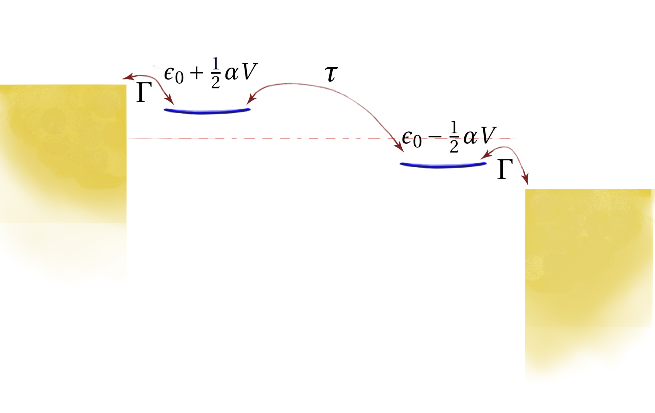
\includegraphics[height=.20\textheight]{pdf/non_interacting_schematics.pdf}\caption{non\hyp{}interacting}\label{fig:twositea}
    \end{subfigure}
    ~
    \begin{subfigure}[b]{0.48\textwidth}
        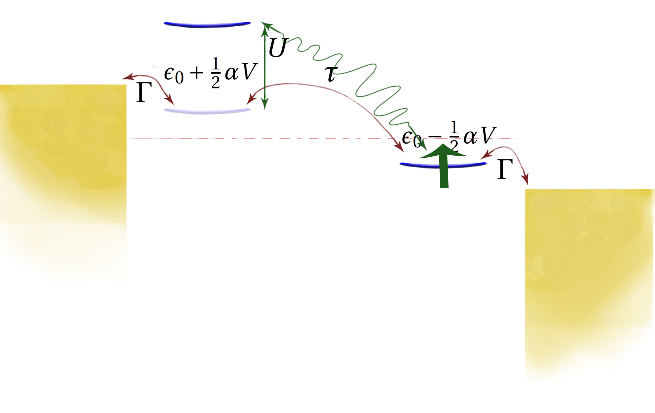
\includegraphics[height=.20\textheight]{pdf/interacting_schematics.pdf}\caption{Interacting}\label{fig:twositeb}
    \end{subfigure}
    \caption{Schematic pictures of the spinless two site model. The red dashed line denotes the Fermi-level. Figure~\ref{fig:twositea} shows the non\hyp{}interacting case, where $\Gamma$ is the molecule-lead coupling, $\epsilon \pm \frac{1}{2} \alpha V$ are the left (right) level and $\tau$ is the tunnelling strength between the levels. In Figure~\ref{fig:twositeb}, an electron (large green arrow) occupies the right level. The swirly line is meant to indicate an interaction with electrons on the left level, thereby raising the level with the capacitive interaction or charging energy $U$.} \label{fig:twosite}
\end{figure}

When no capacitive interaction is included (i.e. $U=0$), the common method (section~\ref{sec:synthesis}) can be applied to find the transmission analytically: \cite{perrinnano}\footnote{If the bias voltage is assumed to be distributed symmetrically over the leads, then the current can be found analytically as well. However, this serves no purpose in this discussion.}:
\begin{align*}
T(\epsilon) &= \frac{ (2\tau)^2 }{(\frac{\Gamma}{2})^2} \frac{(\frac{\Gamma}{2})^2}{(\epsilon-\epsilon_1)^2 + (\frac{\Gamma}{2})^2}\frac{(\frac{\Gamma}{2})^2}{(\epsilon-\epsilon_2)^2 + (\frac{\Gamma}{2})^2},
\end{align*}
where $\epsilon_{1,2} = \epsilon_0 \pm \frac{1}{2} \Delta$, where $\Delta$ is the level splitting in the presence of bias voltage given by $\Delta = \sqrt{ (\alpha V)^2+ 4\tau^2}$. 

For the two-site model including capacitive interactions, we assume that the chance a many-body state $\ket{\kappa}$ is occupied is proportional to the Boltzmann-factor $e^{ -\beta \braket{ \kappa\left| H \right| \kappa}} Z^{-1}$, where $Z$ is a normalisation constant and $H$ the full Hamiltonian including capacitive interactions.

It is illustrative for the application of the many-body Green's function (equation~\ref{eq:mbgfresult}) to consider the shapes of $G^{\lambda\pm}$. Their most important contribution in this context is simply the thermal average of the capacitive self-energy $\braket{\lambda\left|\Sigma^c\right|\lambda}$. The four $G^{\lambda\pm}$ are:
\begin{align*}
G^{\ket{00}\pm} &= \left[ \epsilon \begin{bmatrix} 1 & 0 \\ 0 & 1 \end{bmatrix} - \begin{bmatrix} \epsilon_0 + \frac{1}{2} \alpha V & -\tau \\
-\tau & \epsilon_0 - \frac{1}{2} \alpha V\end{bmatrix}  \pm \frac{\imath}{2} \begin{pmatrix} \Gamma & 0 \\ 0 & \Gamma \end{pmatrix} \right]^{-1}, \\
G^{\ket{10}\pm} &= \left[ \epsilon \begin{bmatrix} 1 & 0 \\ 0 & 1 \end{bmatrix} - \begin{bmatrix} \epsilon_0 + \frac{1}{2} \alpha V & -\tau \\
-\tau & \epsilon_0 - \frac{1}{2} \alpha V\end{bmatrix} - \begin{pmatrix} 0 & 0 \\ 0 & U \end{pmatrix} \pm \frac{\imath}{2} \begin{pmatrix} \Gamma & 0 \\ 0 & \Gamma \end{pmatrix} \right]^{-1}, \\
G^{\ket{01}\pm} &= \left[ \epsilon \begin{bmatrix} 1 & 0 \\ 0 & 1 \end{bmatrix} - \begin{bmatrix} \epsilon_0 + \frac{1}{2} \alpha V & -\tau \\
-\tau & \epsilon_0 - \frac{1}{2} \alpha V\end{bmatrix} - \begin{pmatrix} U & 0 \\ 0 & 0 \end{pmatrix} \pm \frac{\imath}{2} \begin{pmatrix} \Gamma & 0 \\ 0 & \Gamma \end{pmatrix} \right]^{-1},\\
G^{\ket{11}\pm} &= \left[ \epsilon \begin{bmatrix} 1 & 0 \\ 0 & 1 \end{bmatrix} - \begin{bmatrix} \epsilon_0 + \frac{1}{2} \alpha V & -\tau \\
-\tau & \epsilon_0 - \frac{1}{2} \alpha V\end{bmatrix} - \begin{pmatrix} U & 0 \\ 0 & U \end{pmatrix} \pm \frac{\imath}{2} \begin{pmatrix} \Gamma & 0 \\ 0 & \Gamma \end{pmatrix} \right]^{-1},
\end{align*}
where we see that adding an electron to e.g. $\ket{10}$ would add the energy $\epsilon_2$ and the capacitive interaction energy $U$. We see this quite clearly in the capacitive self-energy contribution of $G^{\ket{10}\pm}$. 

\subsection{Spinfull two site model}
When we include spin in the model, we are essentially keeping two copies of the model and add interaction. There is no spin-flip tunnelling. I use the ordered many-body basis $\left\{ \ket{\uparrow 1}, \ket{\downarrow 1}, \ket{\uparrow 2}, \ket{\downarrow 2}\right\}$. The Hamiltonian is:
\begin{align}
H_1 &= \begin{bmatrix} \epsilon_0 + \frac{1}{2} \alpha V & 0 & -\tau & 0 \\ 0 & \epsilon_0 + \frac{1}{2} \alpha V & 0 & -\tau\\ -\tau & 0 & \epsilon_0 - \frac{1}{2} \alpha V & 0 \\ 0 & -\tau & 0 & \epsilon_0 - \frac{1}{2} \alpha V\end{bmatrix},
\label{eq:spinfullhamiltonian}
\end{align} 
while the coupling matrices are:
\begin{align*}
\Gamma^L &= \begin{bmatrix} \Gamma & 0 & 0 & 0 \\ 0 & \Gamma & 0 & 0 \\ 0 & 0 & 0 & 0 \\  0 & 0 & 0 & 0\end{bmatrix},\\ \Gamma^R &= \begin{bmatrix} 0 & 0 & 0 & 0 \\ 0 & 0 & 0 & 0 \\ 0 & 0 & \Gamma & 0 \\ 0 & 0 & 0 & \Gamma \\ \end{bmatrix},
\end{align*}
and the capacitive self-energy is:
\begin{align*}
\Sigma^c &= \begin{bmatrix} \zeta U & 0 & 0 & 0\\ 0 & \zeta U & 0 & 0\\ 0 & 0 & 0 & 0\\ 0 & 0 & 0 & \xi U \end{bmatrix} n_{\uparrow 2} + \begin{bmatrix} \zeta U & 0 & 0 & 0\\ 0 & \zeta U & 0 & 0\\ 0 & 0 & \xi U & 0\\ 0 & 0 & 0 & 0 \end{bmatrix} n_{\downarrow 2} +\\
&\quad\begin{bmatrix} 0 & 0 & 0 & 0\\ 0 & \xi  U & 0 & 0\\ 0 & 0 & \zeta U & 0\\ 0 & 0 & 0 & \zeta U \end{bmatrix} n_{\uparrow 1} + \begin{bmatrix} \xi  U & 0 & 0 & 0\\ 0 & 0 & 0 & 0\\ 0 & 0 & \zeta U & 0\\ 0 & 0 & 0 & \zeta U \end{bmatrix} n_{\downarrow 1},
\end{align*}
where $\zeta U$ describes the strength of capacitive interaction between the left and right site (intersite), whereas $\xi U$ describes the strength of capacitive interaction on the left or right site (onsite).

The definitions for the coupling matrices $\Gamma^{R,L}$ allow us to directly calculate the transmission analytically in terms of the retarded and advanced Green's Function:
\begin{align*}
T(\epsilon) &= \Gamma^2 \left( G^+_{13} G^-_{31} + G^+_{14} G^-_{41} + G^+_{23} G^-_{32} + G^+_{24} G^-_{42} \right),
\end{align*}
where $\Gamma$ is the WBL coupling constant.Note that there is in principle a maximum of $4$ peaks. Because $\left(G^+\right)_{ij}^\star = G^-_{ji}$ in the energy-domain, there is no quantum interference and the function is real valued, as it should be.

\section{Expectations}
\label{sec:expectations}
\subsection{Spinless two-site model}
In section~\ref{sec:twositetransmission}, I will look at selected transmission figures for $U=0.0, 0.05, 0.15$ and $0.5$. The many-body character of the new theory makes it imperative to look at the many-body energies before I can make predictions about the different figures. Recall that the low-temperature Boltzmann distribution specifies that only the lowest-energy many-body state is occupied.
\begin{figure}[!bt]
    \centering
    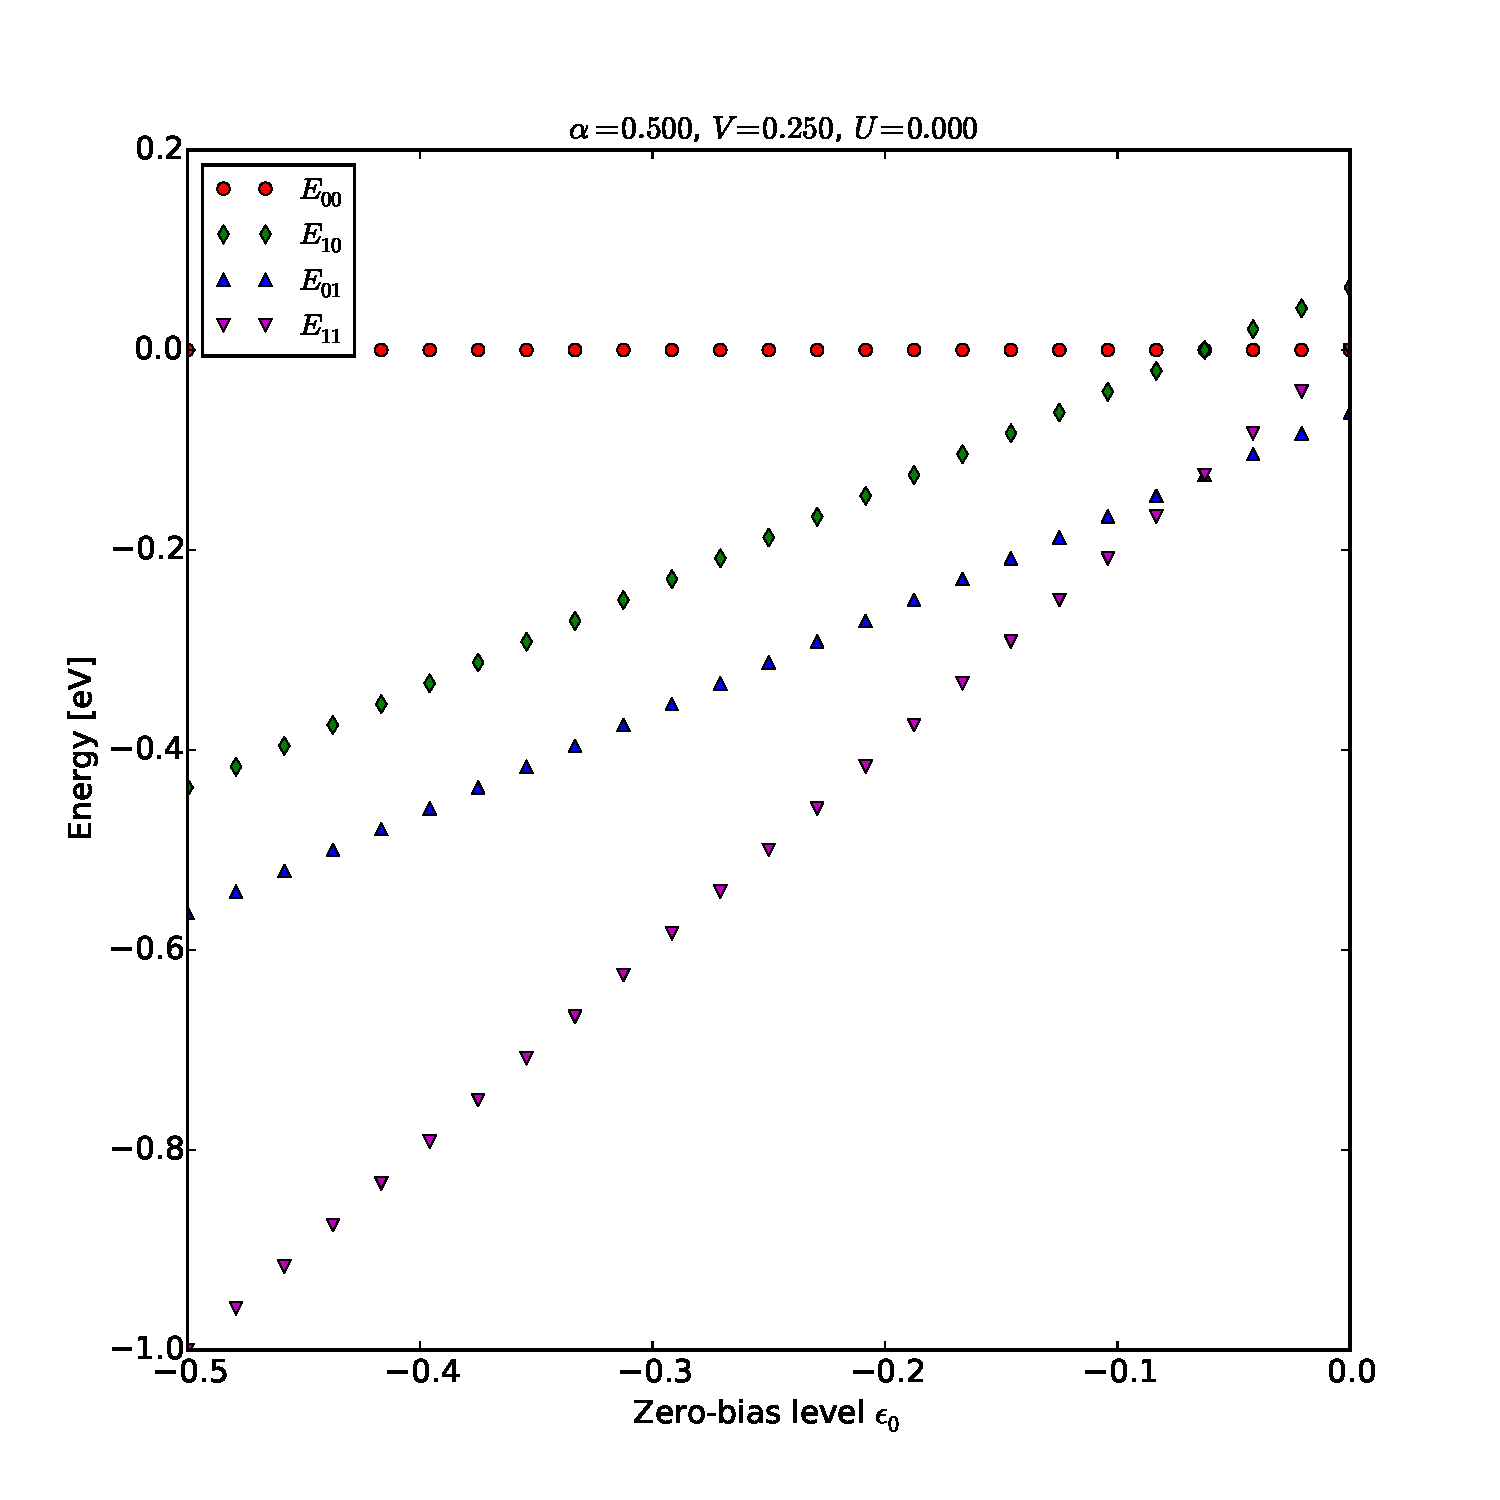
\includegraphics[height=.45\textheight]{pdf/energy/perrin_distribution_u0.pdf}
    \caption{Energy for the spinless two-site model at $U=0$. The subscripts $E_{ij}$ refer to the many-body state $\ket{i j}$. At $\epsilon_0 \approx 0$, there is one electron on the right level. Lowering $\epsilon_0$ past ~$-0.08$ indicates a shift to an occupation of both the left and right levels.  }
    \label{fig:perrinenergy0}
\end{figure}
\begin{figure}[!bt]
    \centering
    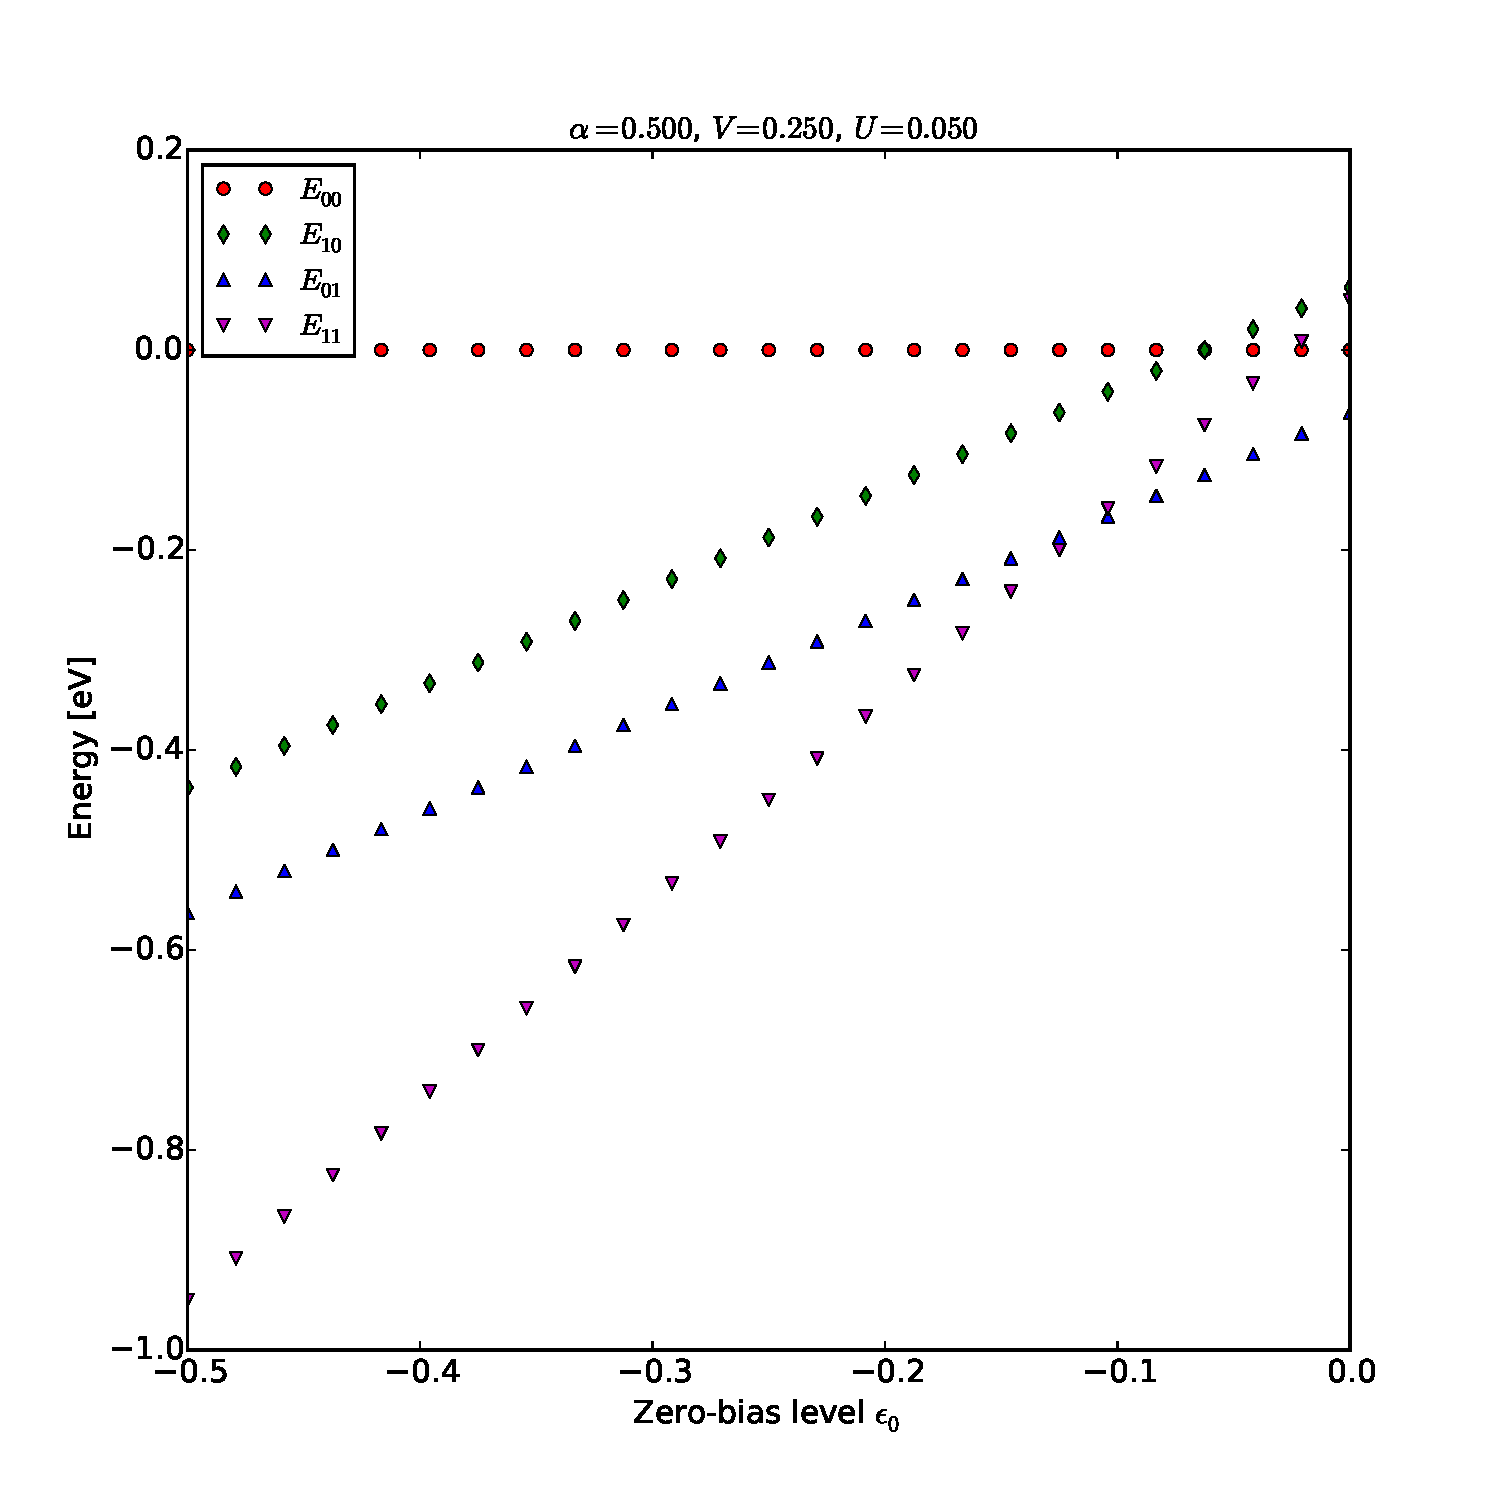
\includegraphics[height=.45\textheight]{pdf/energy/perrin_distribution_u1.pdf}
    \caption{Energy for the spinless two-site model at $U=0.05$. The subscripts $E_{ij}$ refer to the many-body state $\ket{i j}$. At $\epsilon_0 \approx 0$, there is one electron on the right level. Lowering $\epsilon_0$ past ~$-0.12$ indicates a shift to an occupation of both the left and right levels.  }
    \label{fig:perrinenergy1}
\end{figure}
\begin{figure}[!bt]
    \centering
    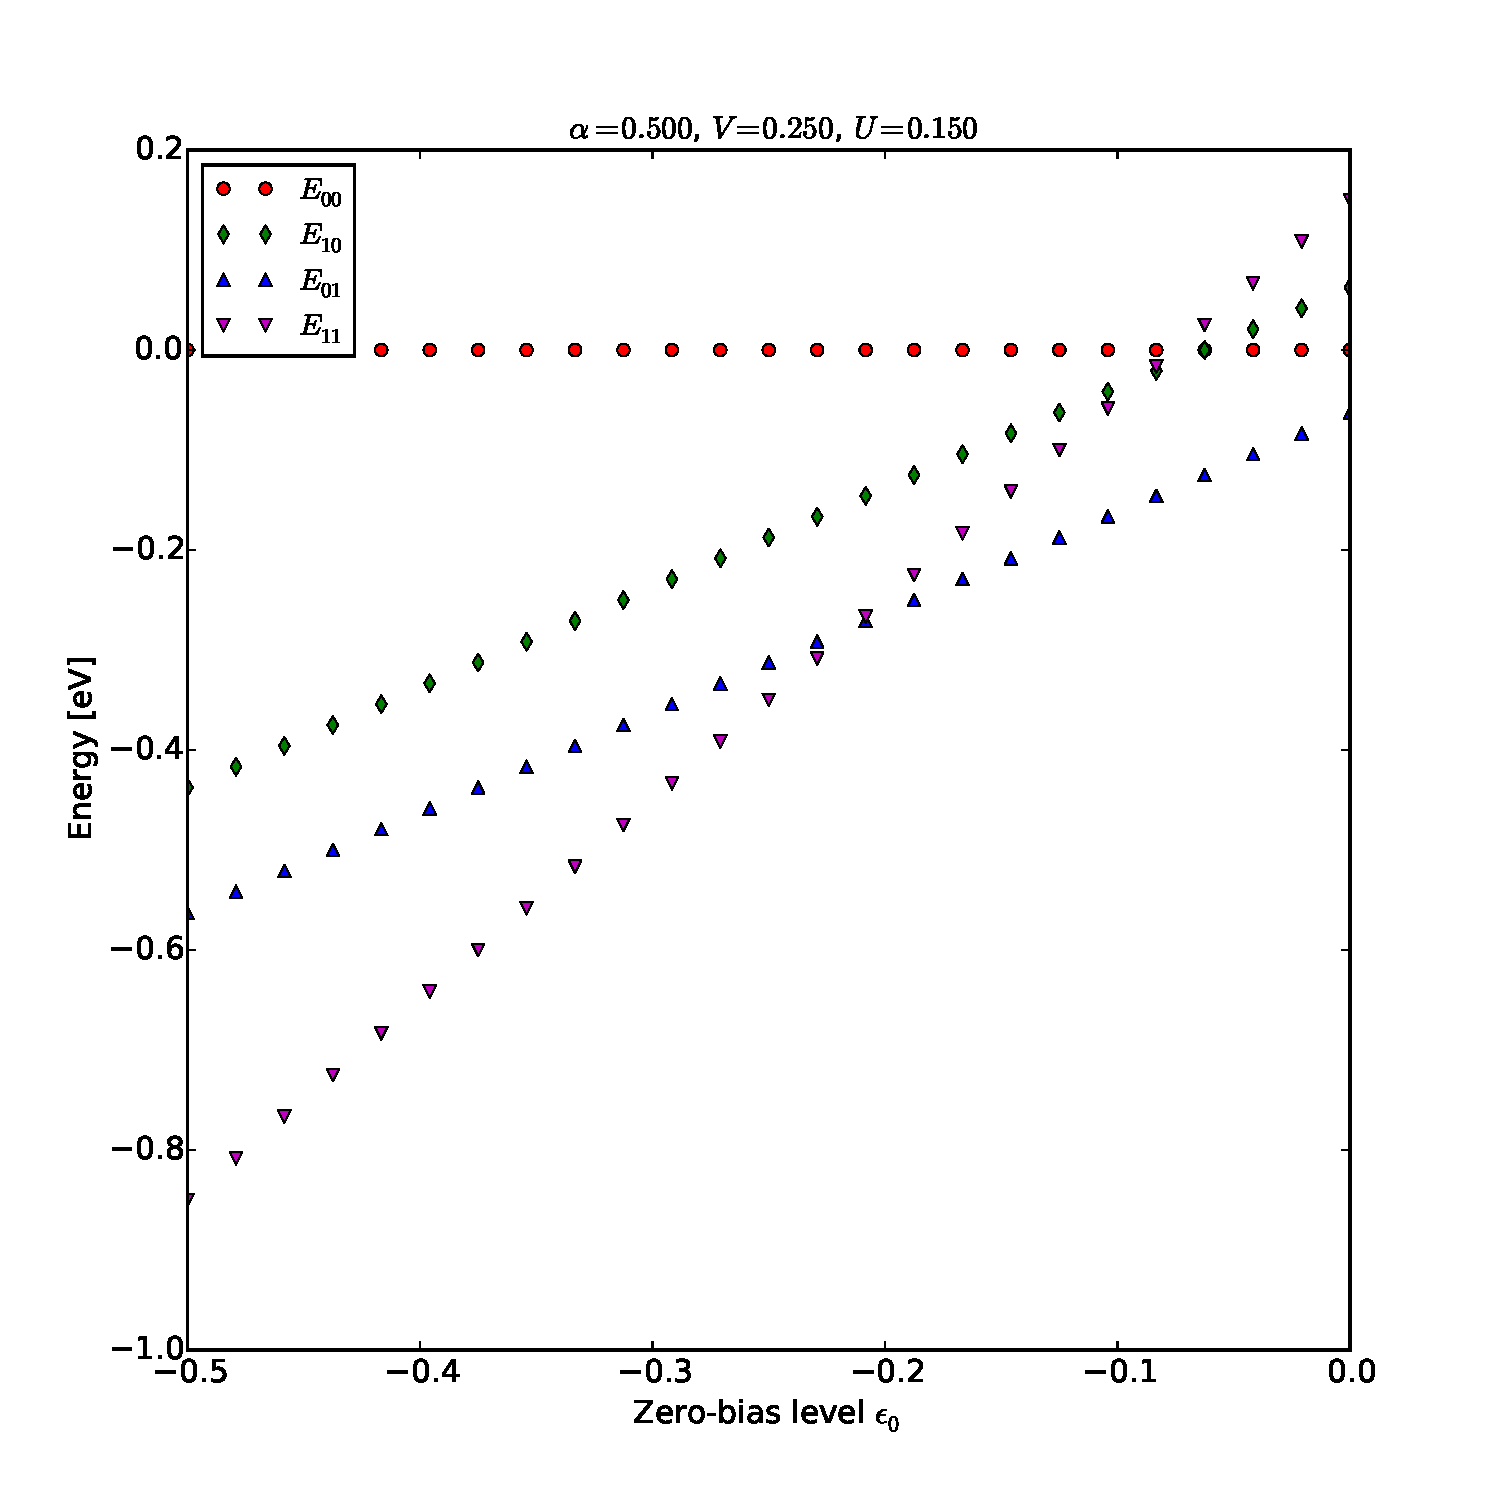
\includegraphics[height=.45\textheight]{pdf/energy/perrin_distribution_u2.pdf}
    \caption{Energy for the spinless two-site model at $U=0.15$. The subscripts $E_{ij}$ refer to the many-body state $\ket{i j}$. At $\epsilon_0 \approx 0$, there is one electron on the right level. Lowering $\epsilon_0$ past ~$-0.23$ indicates a shift to an occupation of both the left and right levels.  }
    \label{fig:perrinenergy2}
\end{figure}
\begin{figure}[!bt]
    \centering
    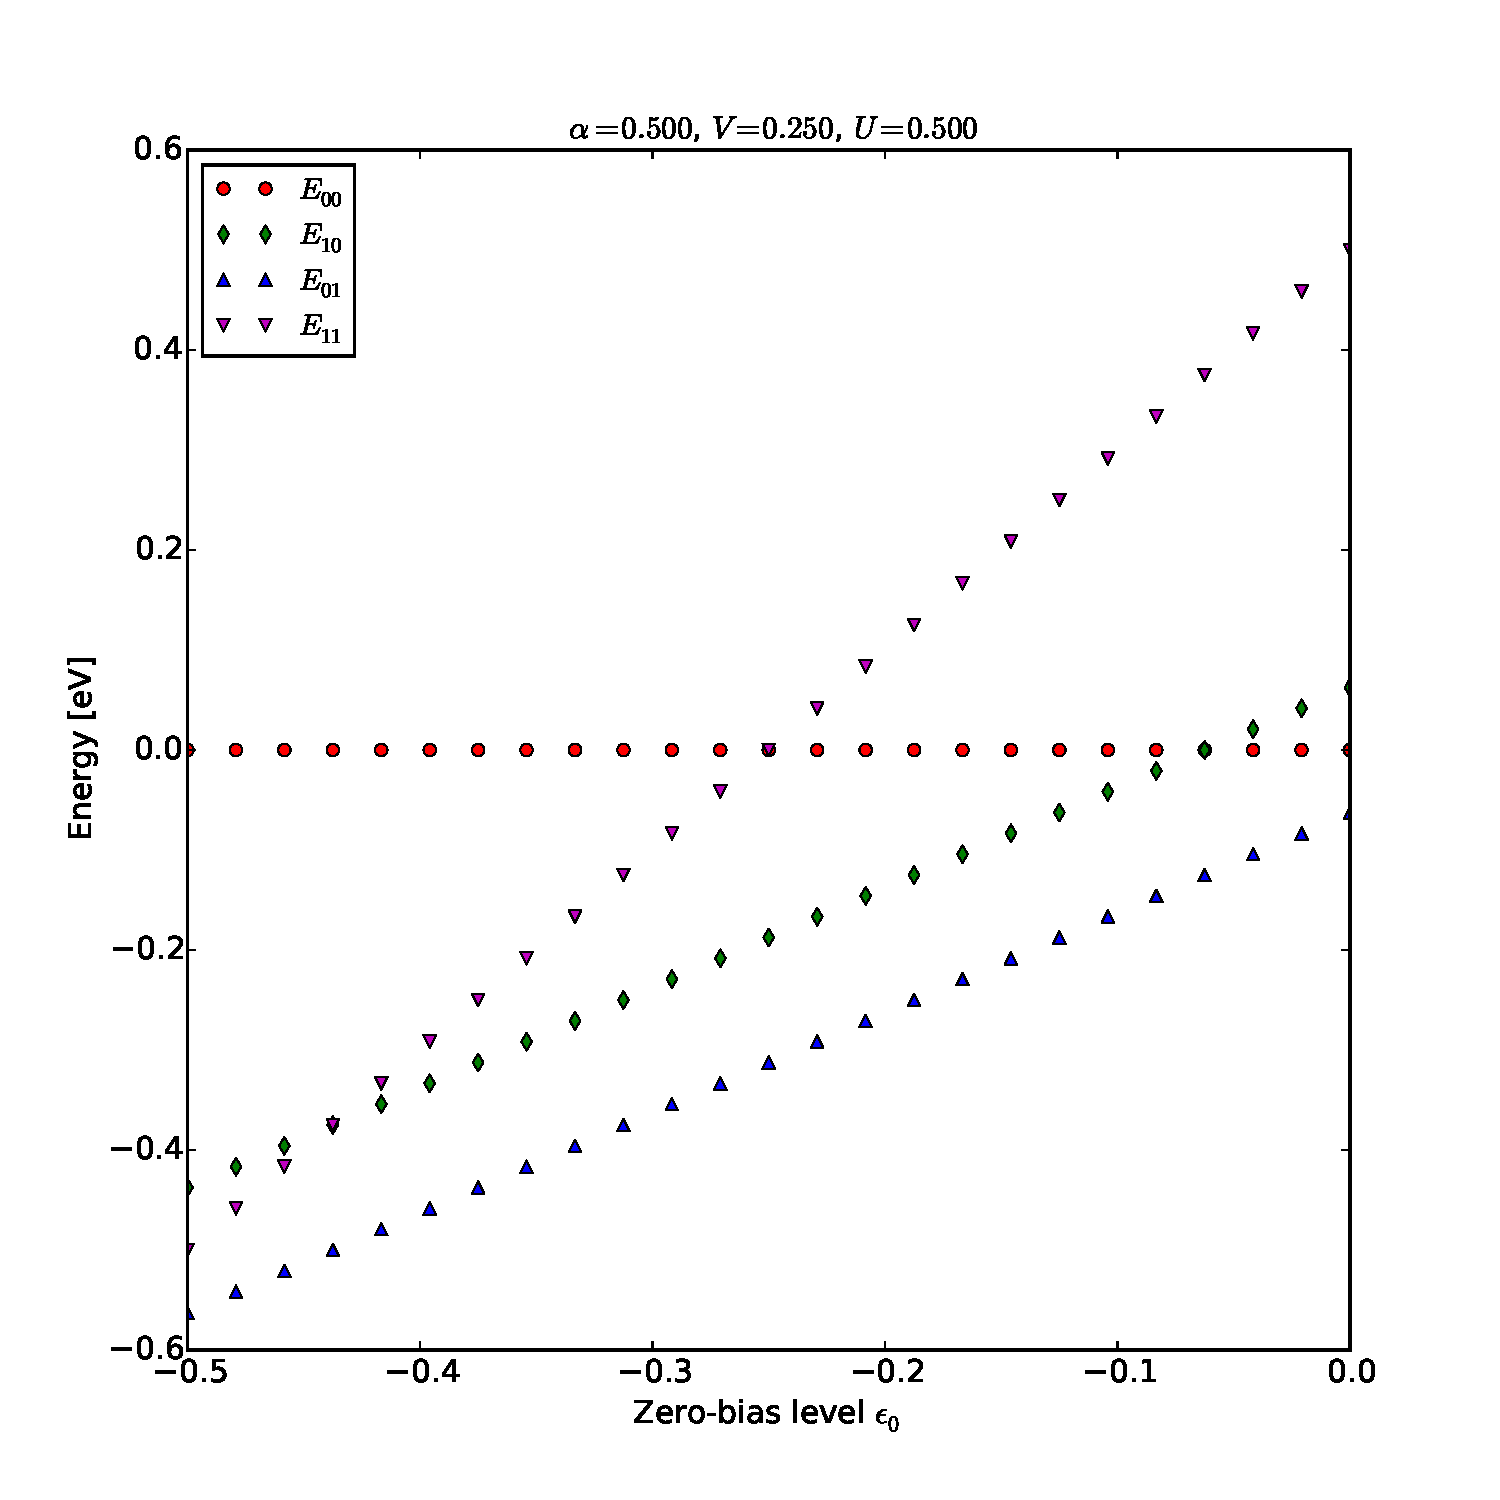
\includegraphics[height=.45\textheight]{pdf/energy/perrin_distribution_u3.pdf}
    \caption{Energy for the spinless two-site model at $U=0.50$. The subscripts $E_{ij}$ refer to the many-body state $\ket{i j}$. At $\epsilon_0 \approx 0$, there is one electron on the right level. Lowering $\epsilon_0$ past ~$-0.58$ indicates a shift to an occupation of both the left and right levels, which is no longer visible in this picture  }
    \label{fig:perrinenergy3}
\end{figure}

Figure~\ref{fig:perrinenergy0} shows the energies for the spinless model when $U=0$, which should be equivalent to the non-interacting model. We see that there is a `switch' from single to double occupation, but this will not cause the capacitive-self energy value to change, because it is zero at $U=0$. In that regard, Figure~\ref{fig:perrinenergy1} is more interesting, as $U=0.05$, causing the switch from $\ket{01}$ to $\ket{11}$ to have not only a different energy, but to cause different transport behaviour. In the first state, there will be one transmission peak at $\epsilon_R$ and one at $\epsilon_L + U$. However, in the second state the second peak is also raised to $\epsilon_R+U$. Since this moves the levels further off-resonance, the transmission peak will be of lower height. The same behaviour persists for Figure~\ref{fig:perrinenergy2} and Figure~\ref{fig:perrinenergy3}, where I note that the switch moves towards lower values of $\epsilon_0$, which is to be expected as the double occupation energy $E_{11} = 2\epsilon_0 + U$ - higher capacitive interaction strength will raise the double occupation energy.
 
\subsection{Spinfull two-site model} 
In this section, I present the energies of the spinfull model at $U=0.0, 0.05, 0.15$ and $0.5$. The parameters $\zeta,\xi$ greatly increase the parameter space for these figures. Here, I will present only the results for $\zeta=1.0$ and the combinations $(U, \xi) = (0.0, 0.0), (0.05, 1.0), (0.15, 1.00), (0.5, 0.50), (0.5, 20.0)$. These are selected to match the transmission figures presented in section~\ref{sec:twositetransmission}.

The Fock-space of occupation states for the spinfull model has dimension $2^4$, so that the figures are full of information. 
\begin{figure}[!bt]
    \centering
    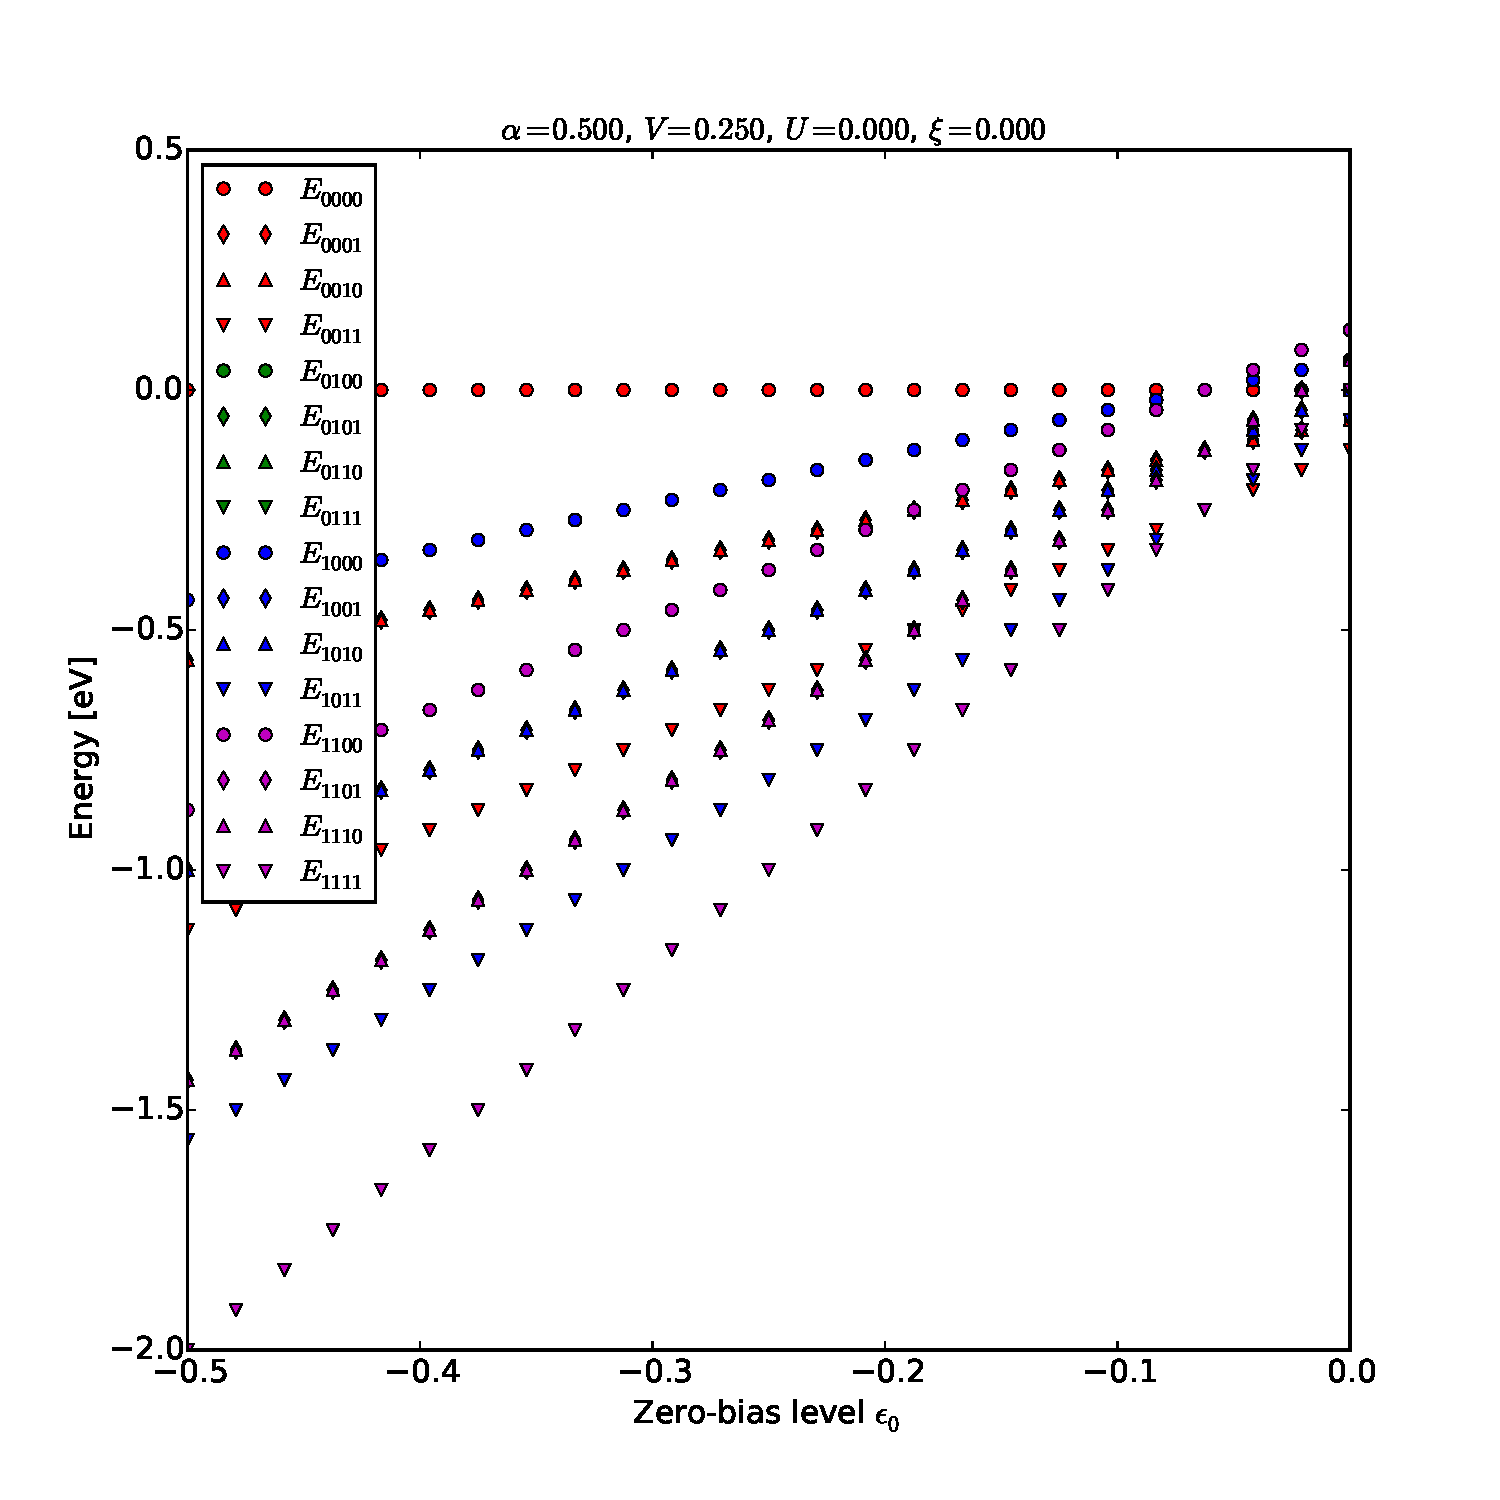
\includegraphics[height=.45\textheight]{pdf/energy/pespin_distribution_u0_k0.pdf}
    \caption{The energy $E_{ijkl}$ denotes the energy for the state $\ket{ijkl}$. In this figure, $U=0.00, \zeta=1.00, \xi=0.00$. The lowest energy state is $\ket{0011}$ for $\epsilon_0\gtrsim -0.18$, which then switches to $\ket{1011}$ or $\ket{0111}$. Then, as $\epsilon_0 \lesssim -.23$ there is a switch to $\ket{1111}$.}
    \label{fig:perspinenergy00}
\end{figure} 
\begin{figure}[!bt]
    \centering
    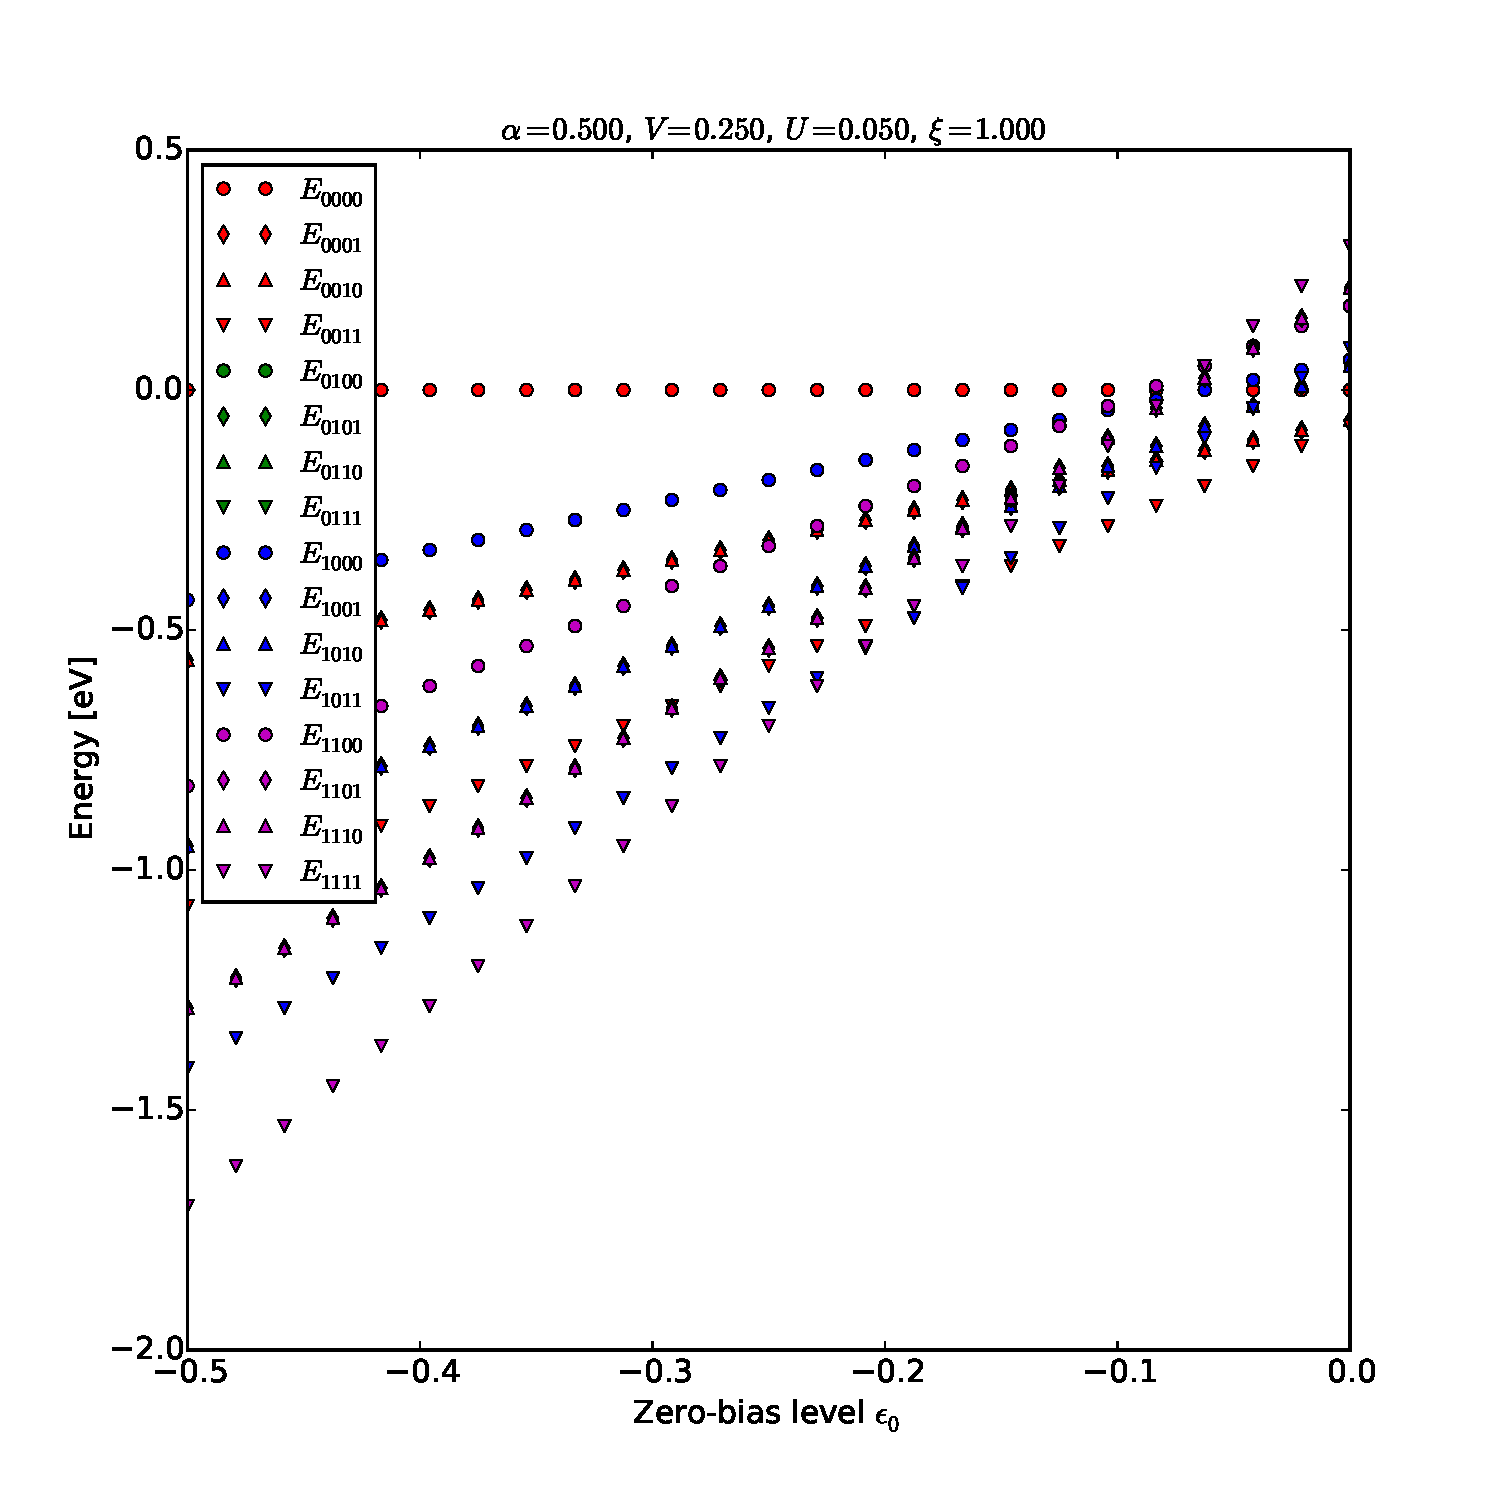
\includegraphics[height=.45\textheight]{pdf/energy/pespin_distribution_u1_k2.pdf}
    \caption{The energy $E_{ijkl}$ denotes the energy for the state $\ket{ijkl}$. In this figure, $U=0.05, \zeta=1.00, \xi=1.00$. The lowest energy state is $\ket{0011}$ for $\epsilon_0\gtrsim -0.15$, which then switches to $\ket{1111}$.}
    \label{fig:perspinenergy12}
\end{figure} 
\begin{figure}[!bt]
    \centering
    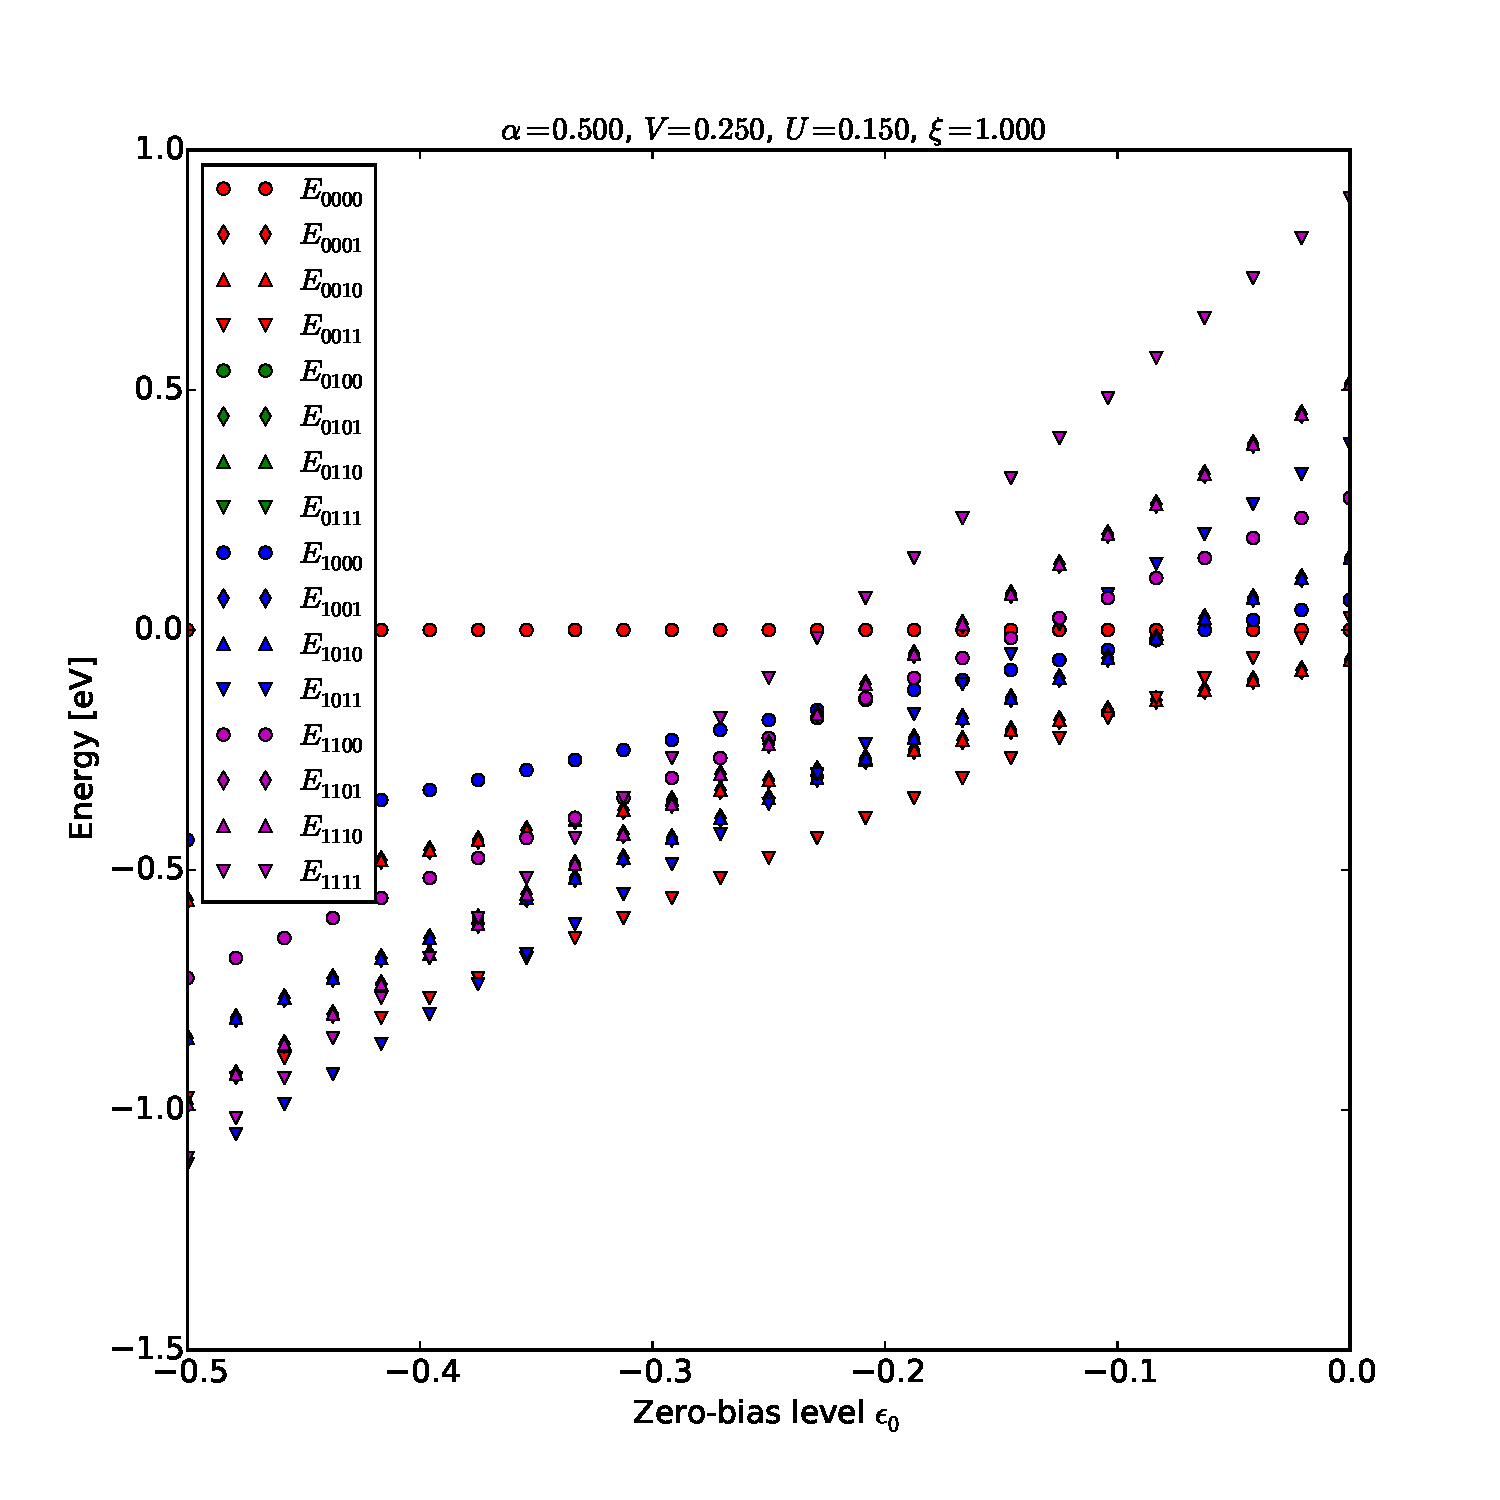
\includegraphics[height=.45\textheight]{pdf/energy/pespin_distribution_u2_k2.pdf}
    \caption{The energy $E_{ijkl}$ denotes the energy for the state $\ket{ijkl}$. In this figure, $U=0.15, \zeta=1.00, \xi=1.00$. The lowest energy state is $\ket{0001}$ or $\ket{0010}$ for $\epsilon_0\gtrsim -0.11$, which then switches to $\ket{0011}$ until $\epsilon_0\lesssim -0.33$ after which it is $\ket{1011}$ or $\ket{0111}$.}
    \label{fig:perspinenergy22}
\end{figure} 
\begin{figure}[!bt]
    \centering
    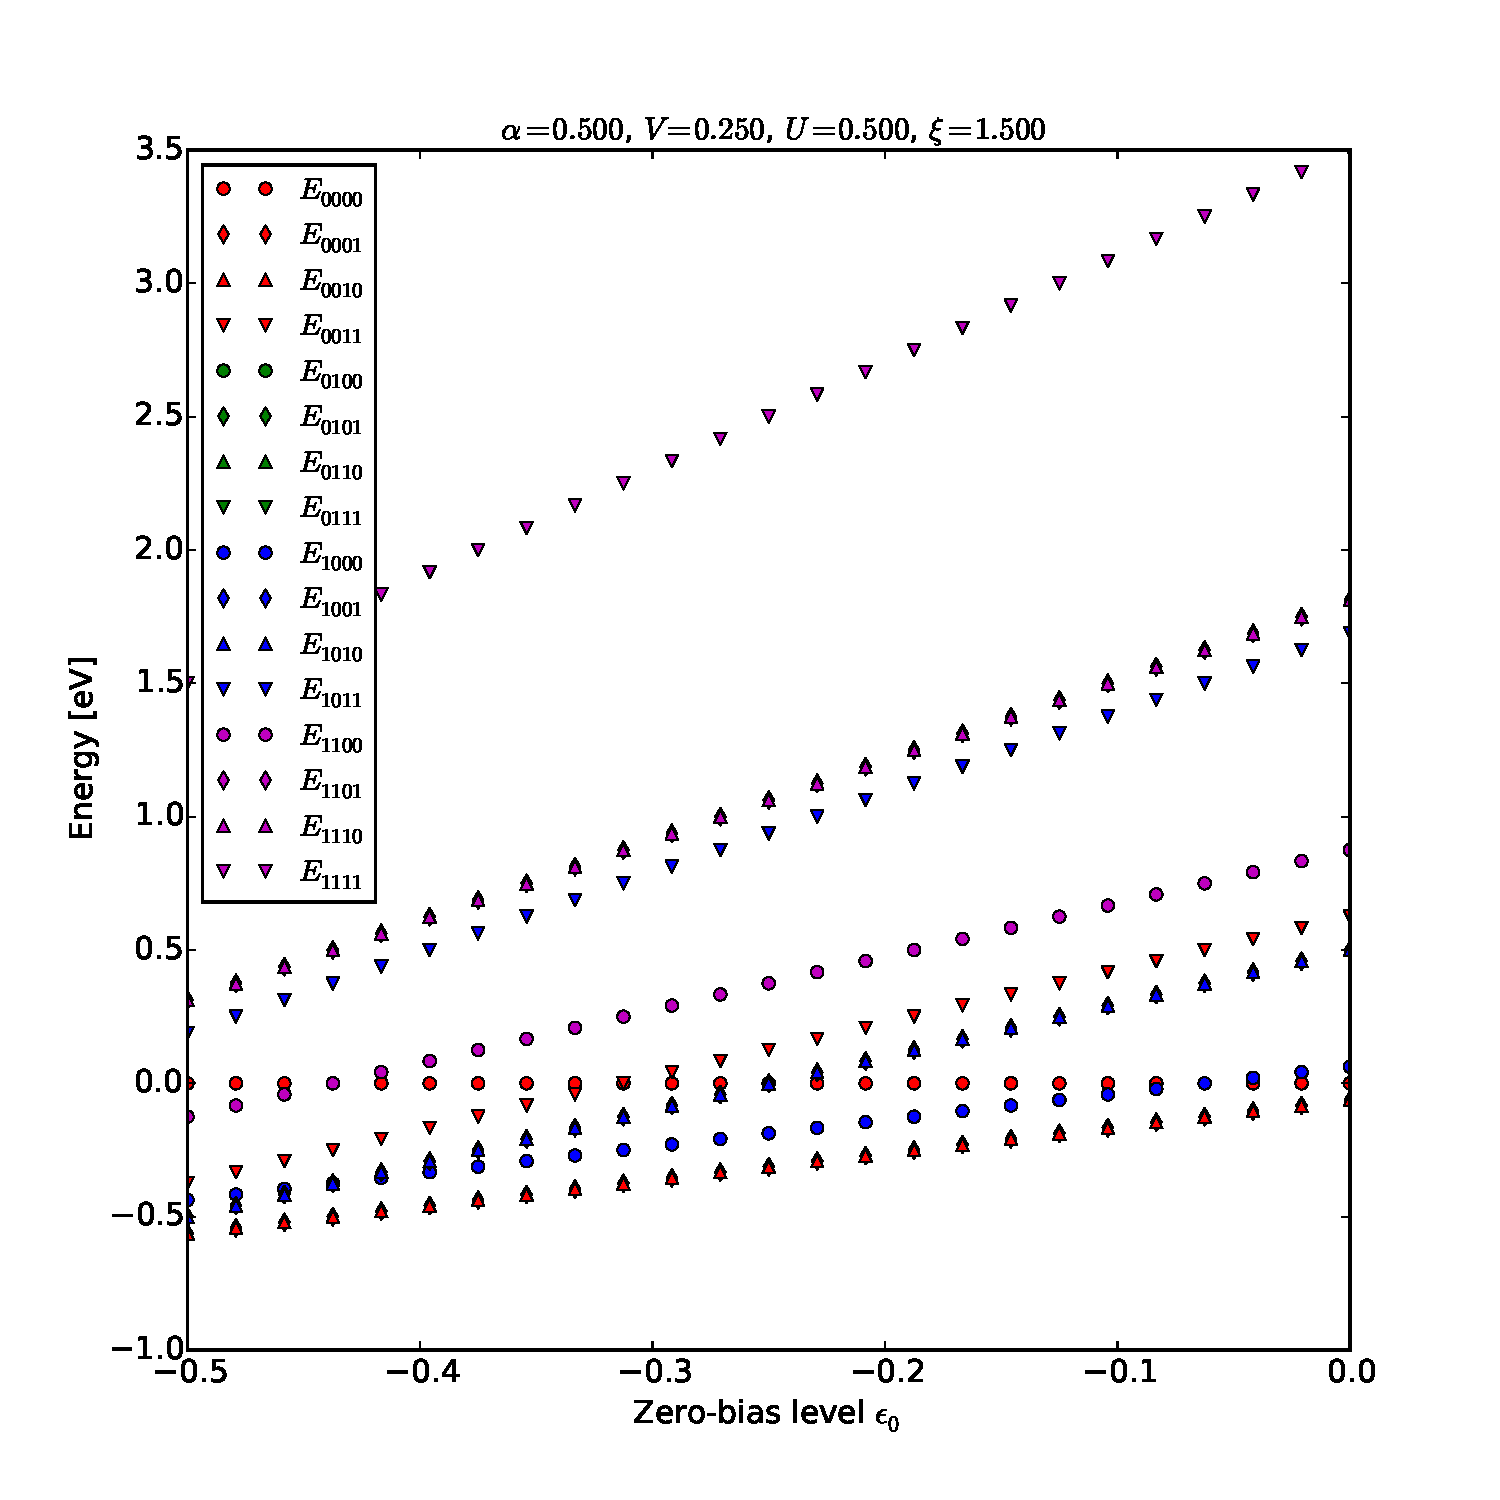
\includegraphics[height=.45\textheight]{pdf/energy/pespin_distribution_u3_k3.pdf}
    \caption{The energy $E_{ijkl}$ denotes the energy for the state $\ket{ijkl}$. In this figure, $U=0.5, \zeta=1.00, \xi=1.50$. The lowest energy state is $\ket{0001}$ or $\ket{0010}$ for all visible $\epsilon_0$.}
    \label{fig:perspinenergy33}
\end{figure} 
\begin{figure}[!bt]
    \centering
    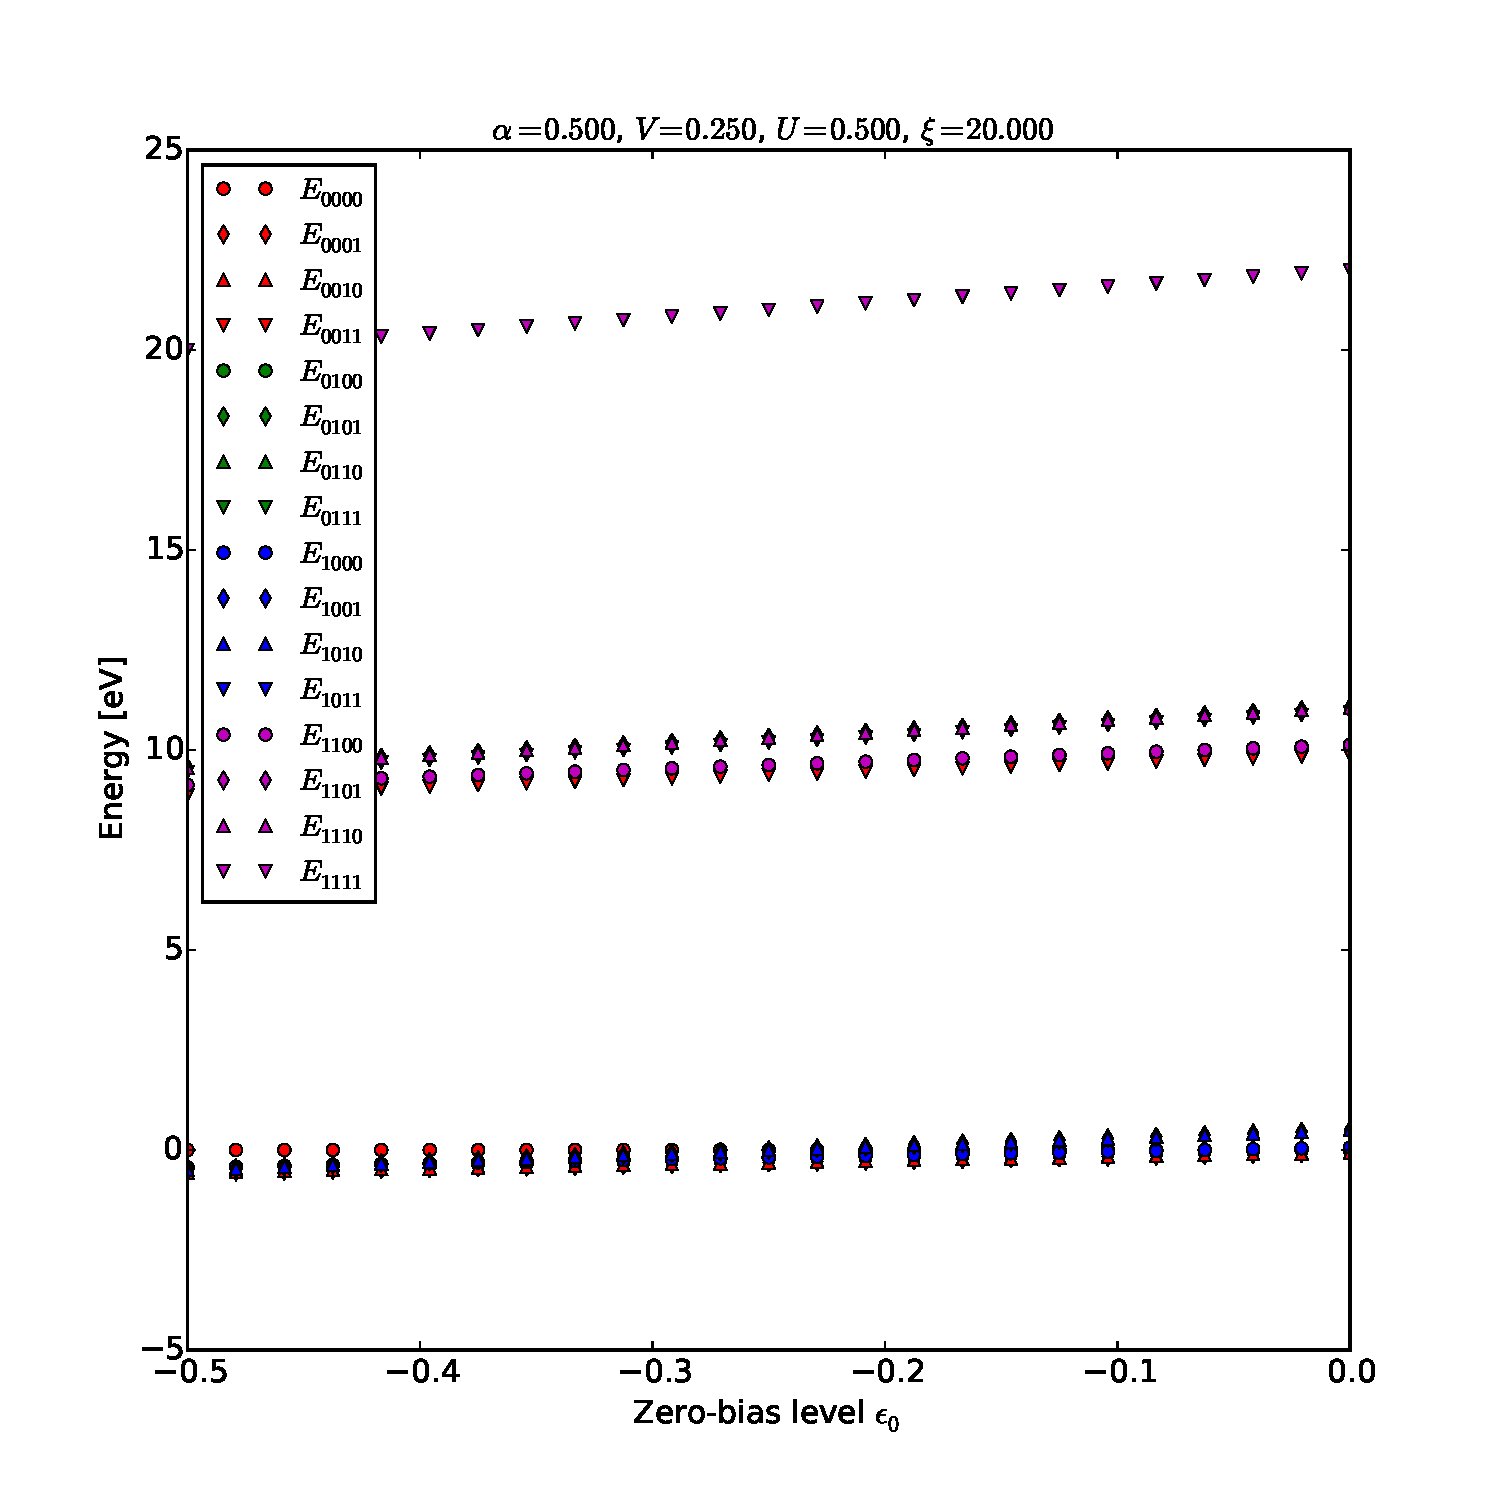
\includegraphics[height=.45\textheight]{pdf/energy/pespin_distribution_u3_k4.pdf}
    \caption{The energy $E_{ijkl}$ denotes the energy for the state $\ket{ijkl}$. In this figure, $U=0.5, \zeta=1.00, \xi=20.0$. The lowest energy state is $\ket{0001}$ or $\ket{0010}$ for all visible $\epsilon_0$.}
    \label{fig:perspinenergy34}
\end{figure}

In Figures~\ref{fig:perspinenergy00},~\ref{fig:perspinenergy12},~\ref{fig:perspinenergy22},~\ref{fig:perspinenergy33},~\ref{fig:perspinenergy34} I see similar behaviour as in the spinless case. There are switches between different many-body states, which are expected to cause some transmission peaks to shift by $\zeta U$ or $\xi U$ or both. The specifics of the many-body states are indicated in their captions.

\section{Transmission}
\label{sec:twositetransmission}
\section{Spinless two-site model}
First, I want to look at the transmission for the spinless model. In Figure~\ref{fig:spinlesstransmissionu0} the non\hyp{}interacting transmission ($U=0$) for otherwise arbitrary but physical parameters is depicted. As you can see, the transmission peaks are exactly at the eigenvalues of the lead-molecule Hamiltonian $H_1 + H_\tau$. If I increase the capacitive interaction strength to $U=0.05$, depicted in Figure~\ref{fig:spinlesstransmissionu1}, two things happen. The peak value of $T(\epsilon)$ reduces from $.16$ to $.13$, because the sites are further removed from resonance. The second transmission peak shifts slightly to the right and is exactly $U$ removed from the corresponding eigenvalue. Further increasing $U$ to e.g. $U=0.5$ in Figure~\ref{fig:spinlesstransmissionu4} yields a more pronounced effect, which is otherwise the same; the peak height reduces and the rightmost peak is exactly $U$ removed from the corresponding eigenvalue.
\begin{figure}[!bt]
    \centering
    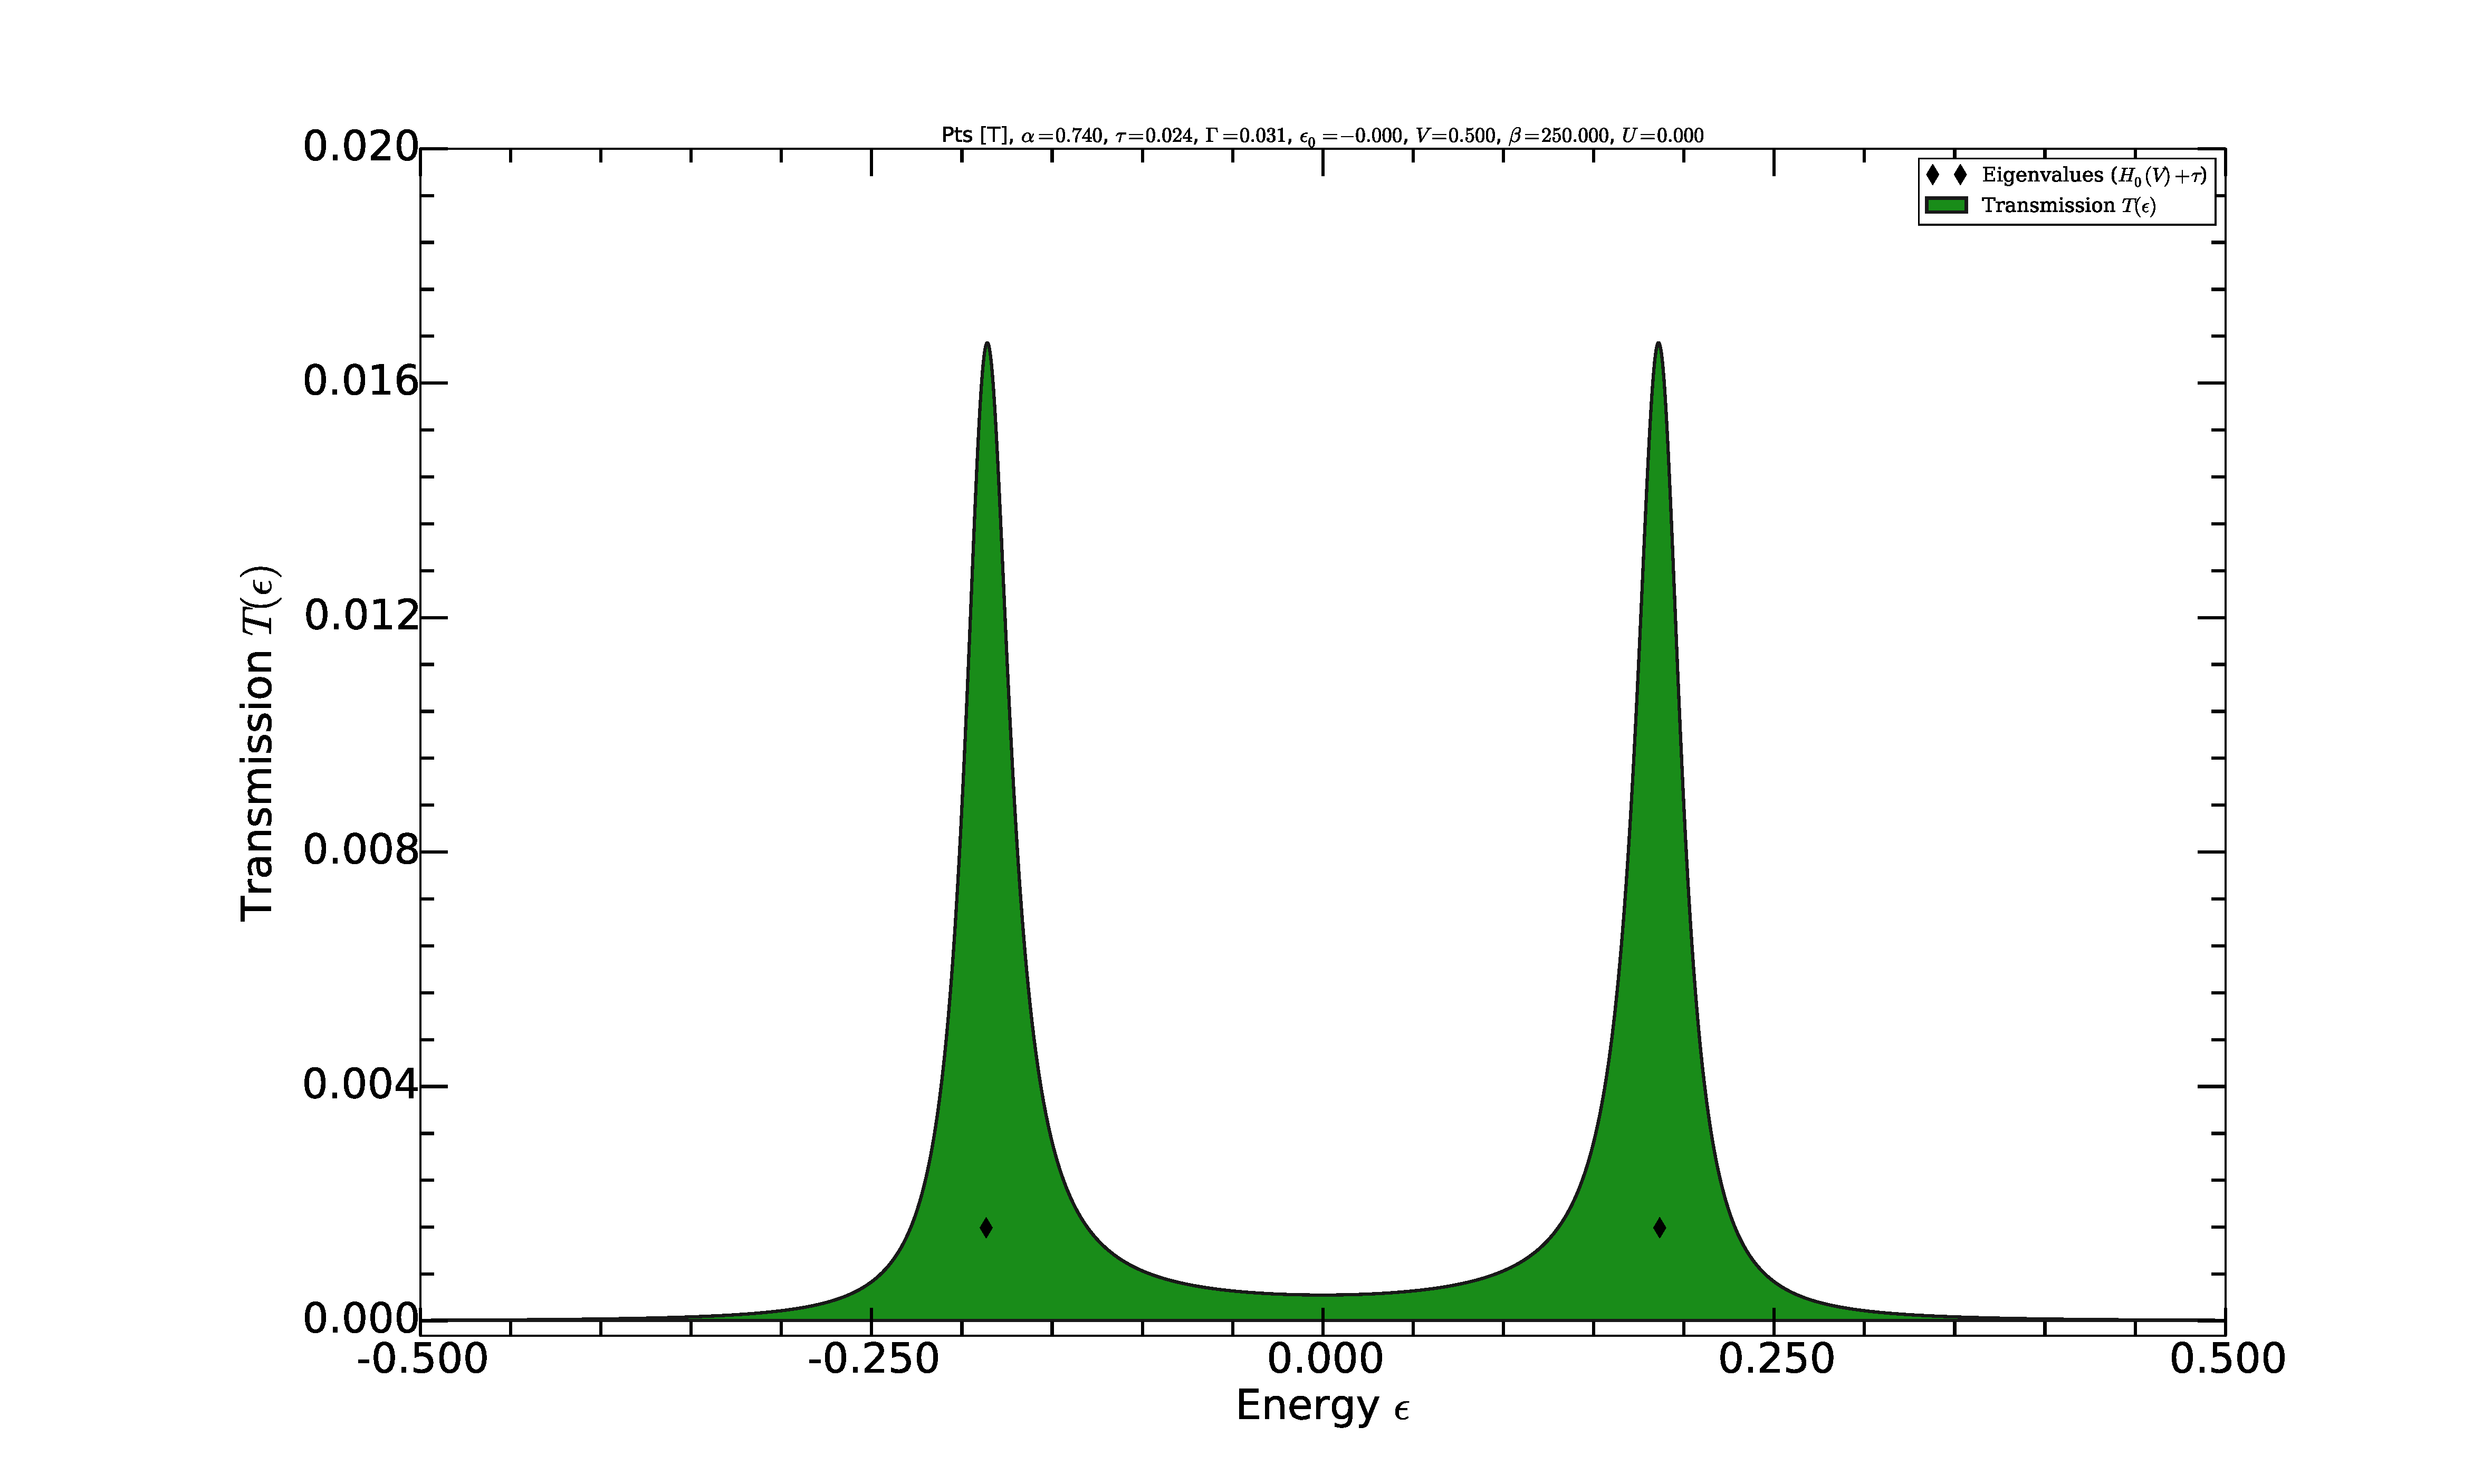
\includegraphics[height=.35\textheight,clip=true,trim=7cm 2cm 7cm 4cm]{pdf/trans/decospinlesstransmissionarbitraryu0.pdf}
    \caption{Transmission spectra for $\alpha=0.74$, $\tau=0.024$, $\Gamma=0.031$, $\epsilon_0 = - 0.05$, $V=0.50$ and $U=0.0$. This a set of parameters for which the system is non\hyp{}interacting . In this picture, the influence of the Stark effect pulling the levels out of resonance is clear in the reduction of peak height which is unity at zero bias.}
    \label{fig:spinlesstransmissionu0}
\end{figure}
\begin{figure}[!bt]
    \centering
    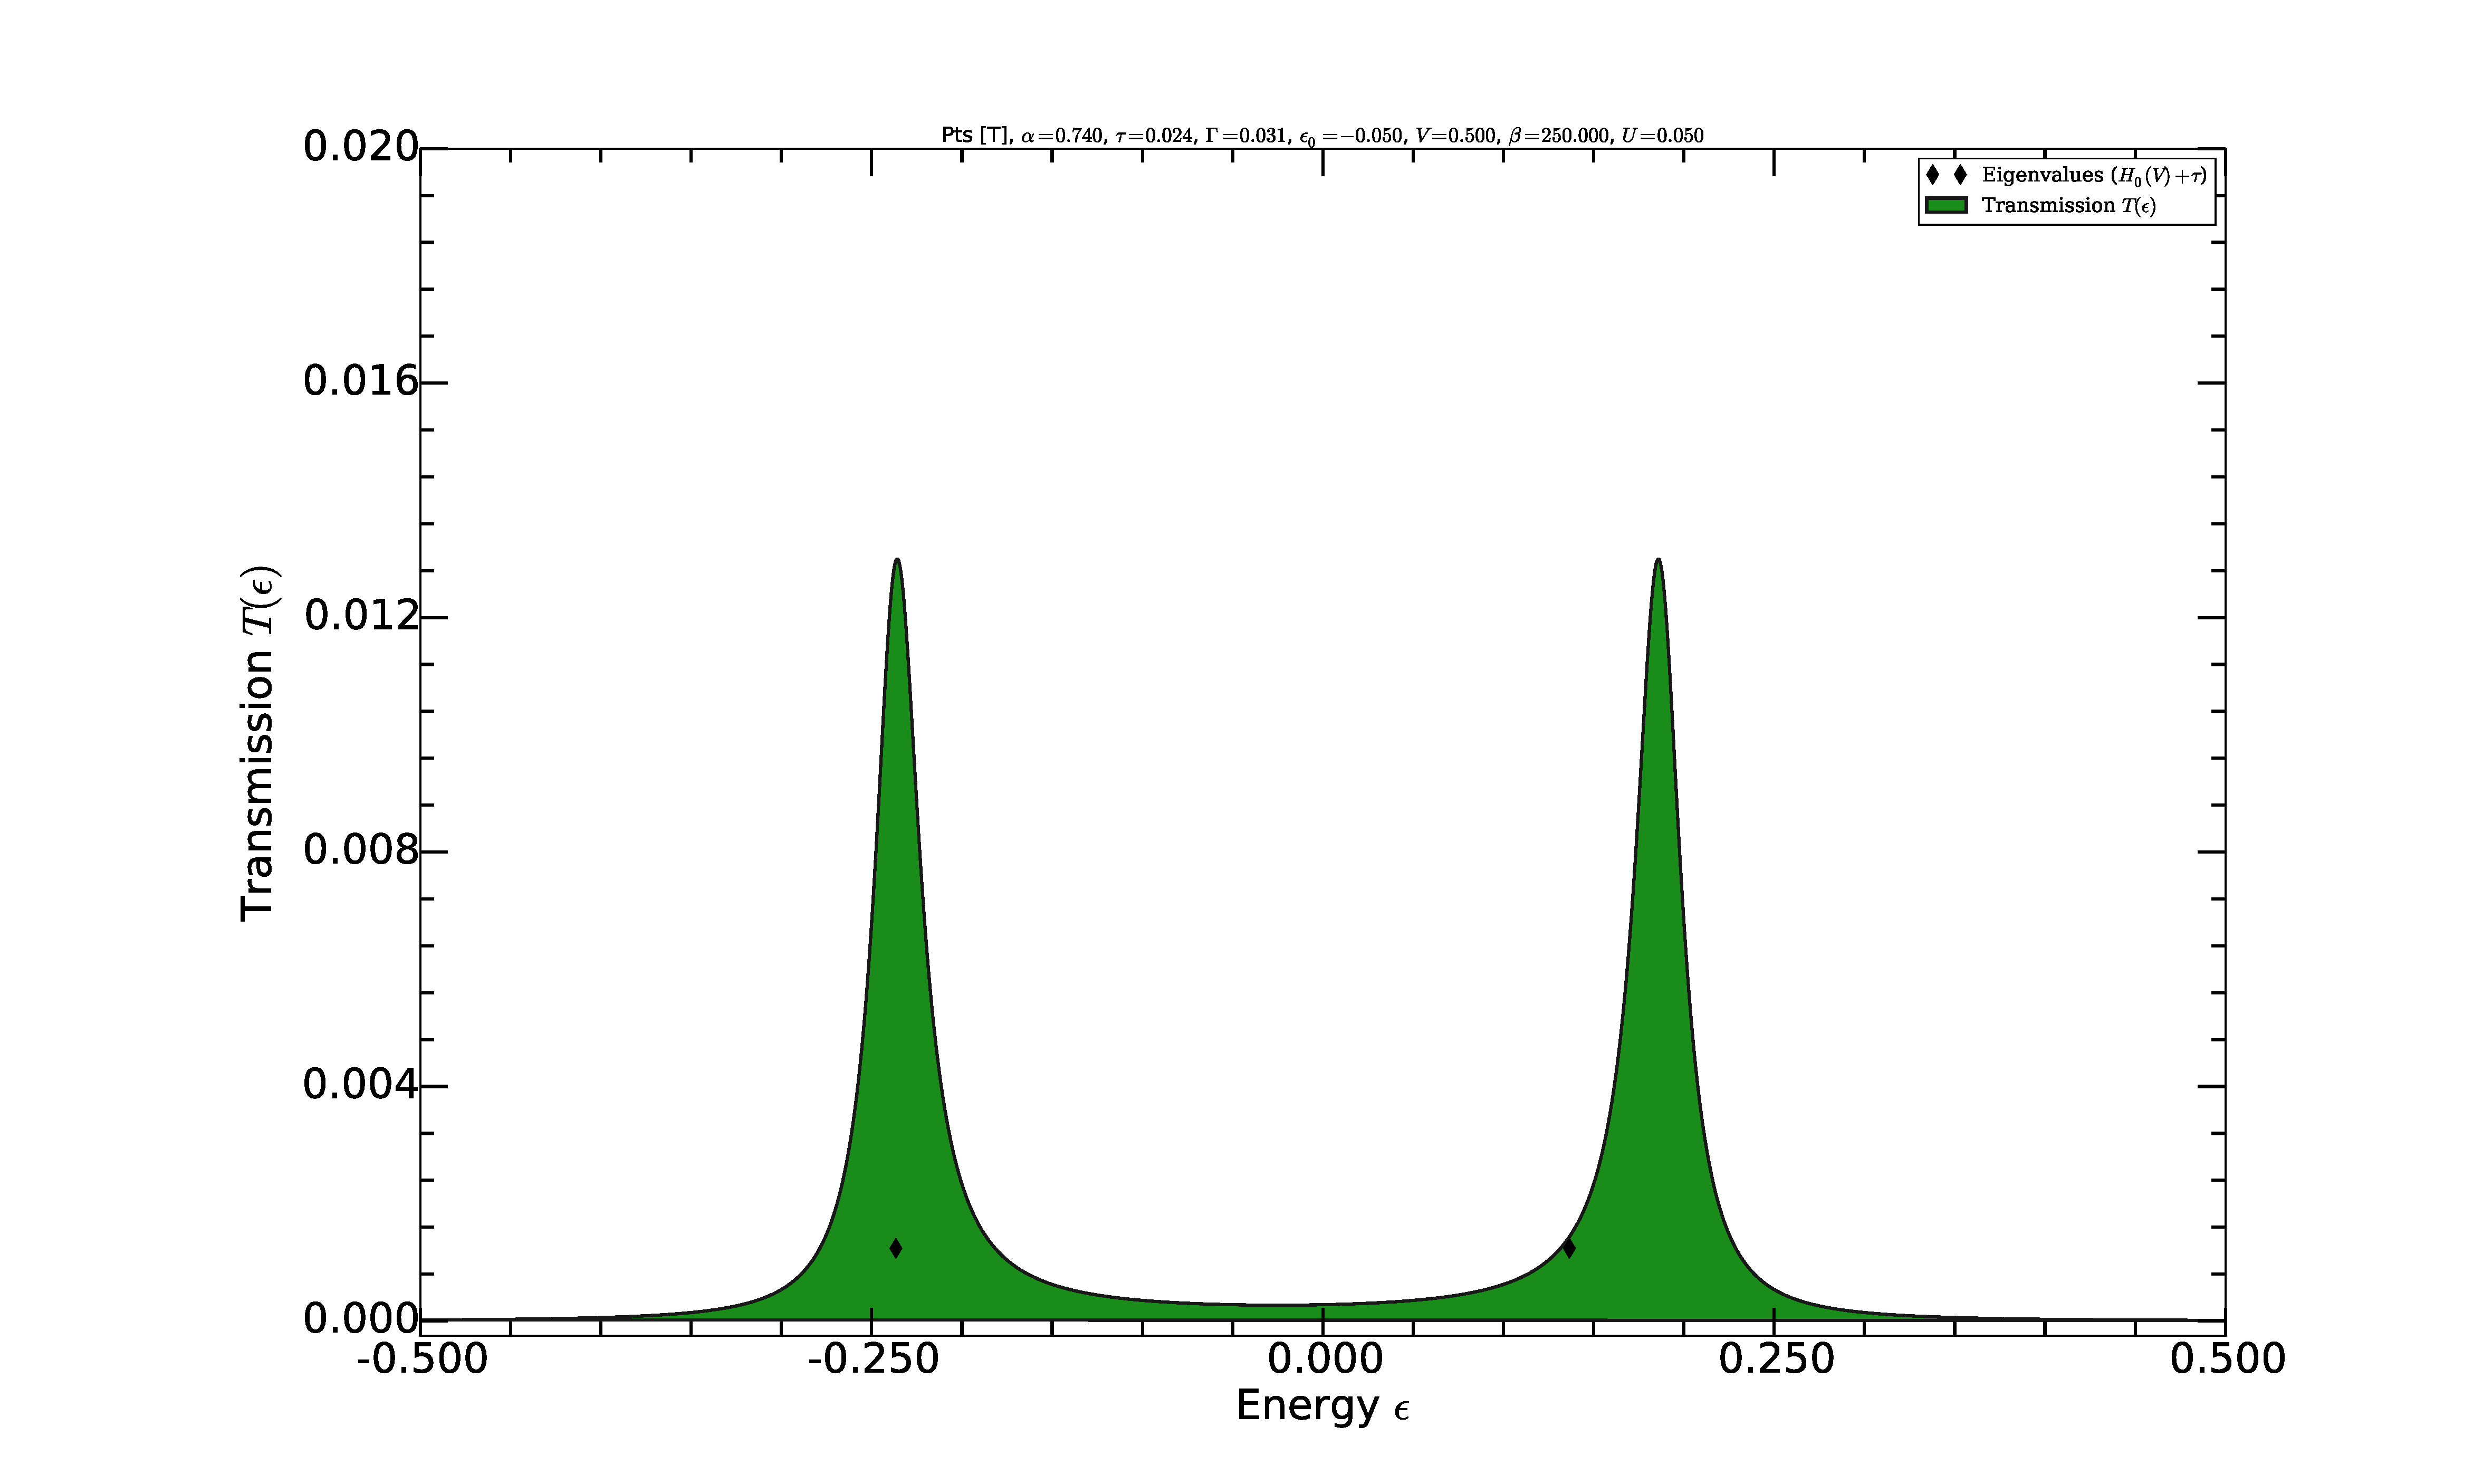
\includegraphics[height=.35\textheight,clip=true,trim=7cm 2cm 7cm 4cm]{pdf/trans/decospinlesstransmissionarbitraryu1.pdf}
    \caption{Transmission spectra for $\alpha=0.74$, $\tau=0.024$, $\Gamma=0.031$, $\epsilon_0 = - 0.05$, $V=0.50$ and $U=0.05$. These parameters indicate a very-weakly interacting system. In comparison to Figure~\ref{fig:spinlesstransmissionu0}, the peak height is smaller and the rightmost peak is clearly displaced from the corresponding eigenvalue (diamond) by $U$. }
    \label{fig:spinlesstransmissionu1}
\end{figure}
\begin{figure}[!bt]
    \centering
    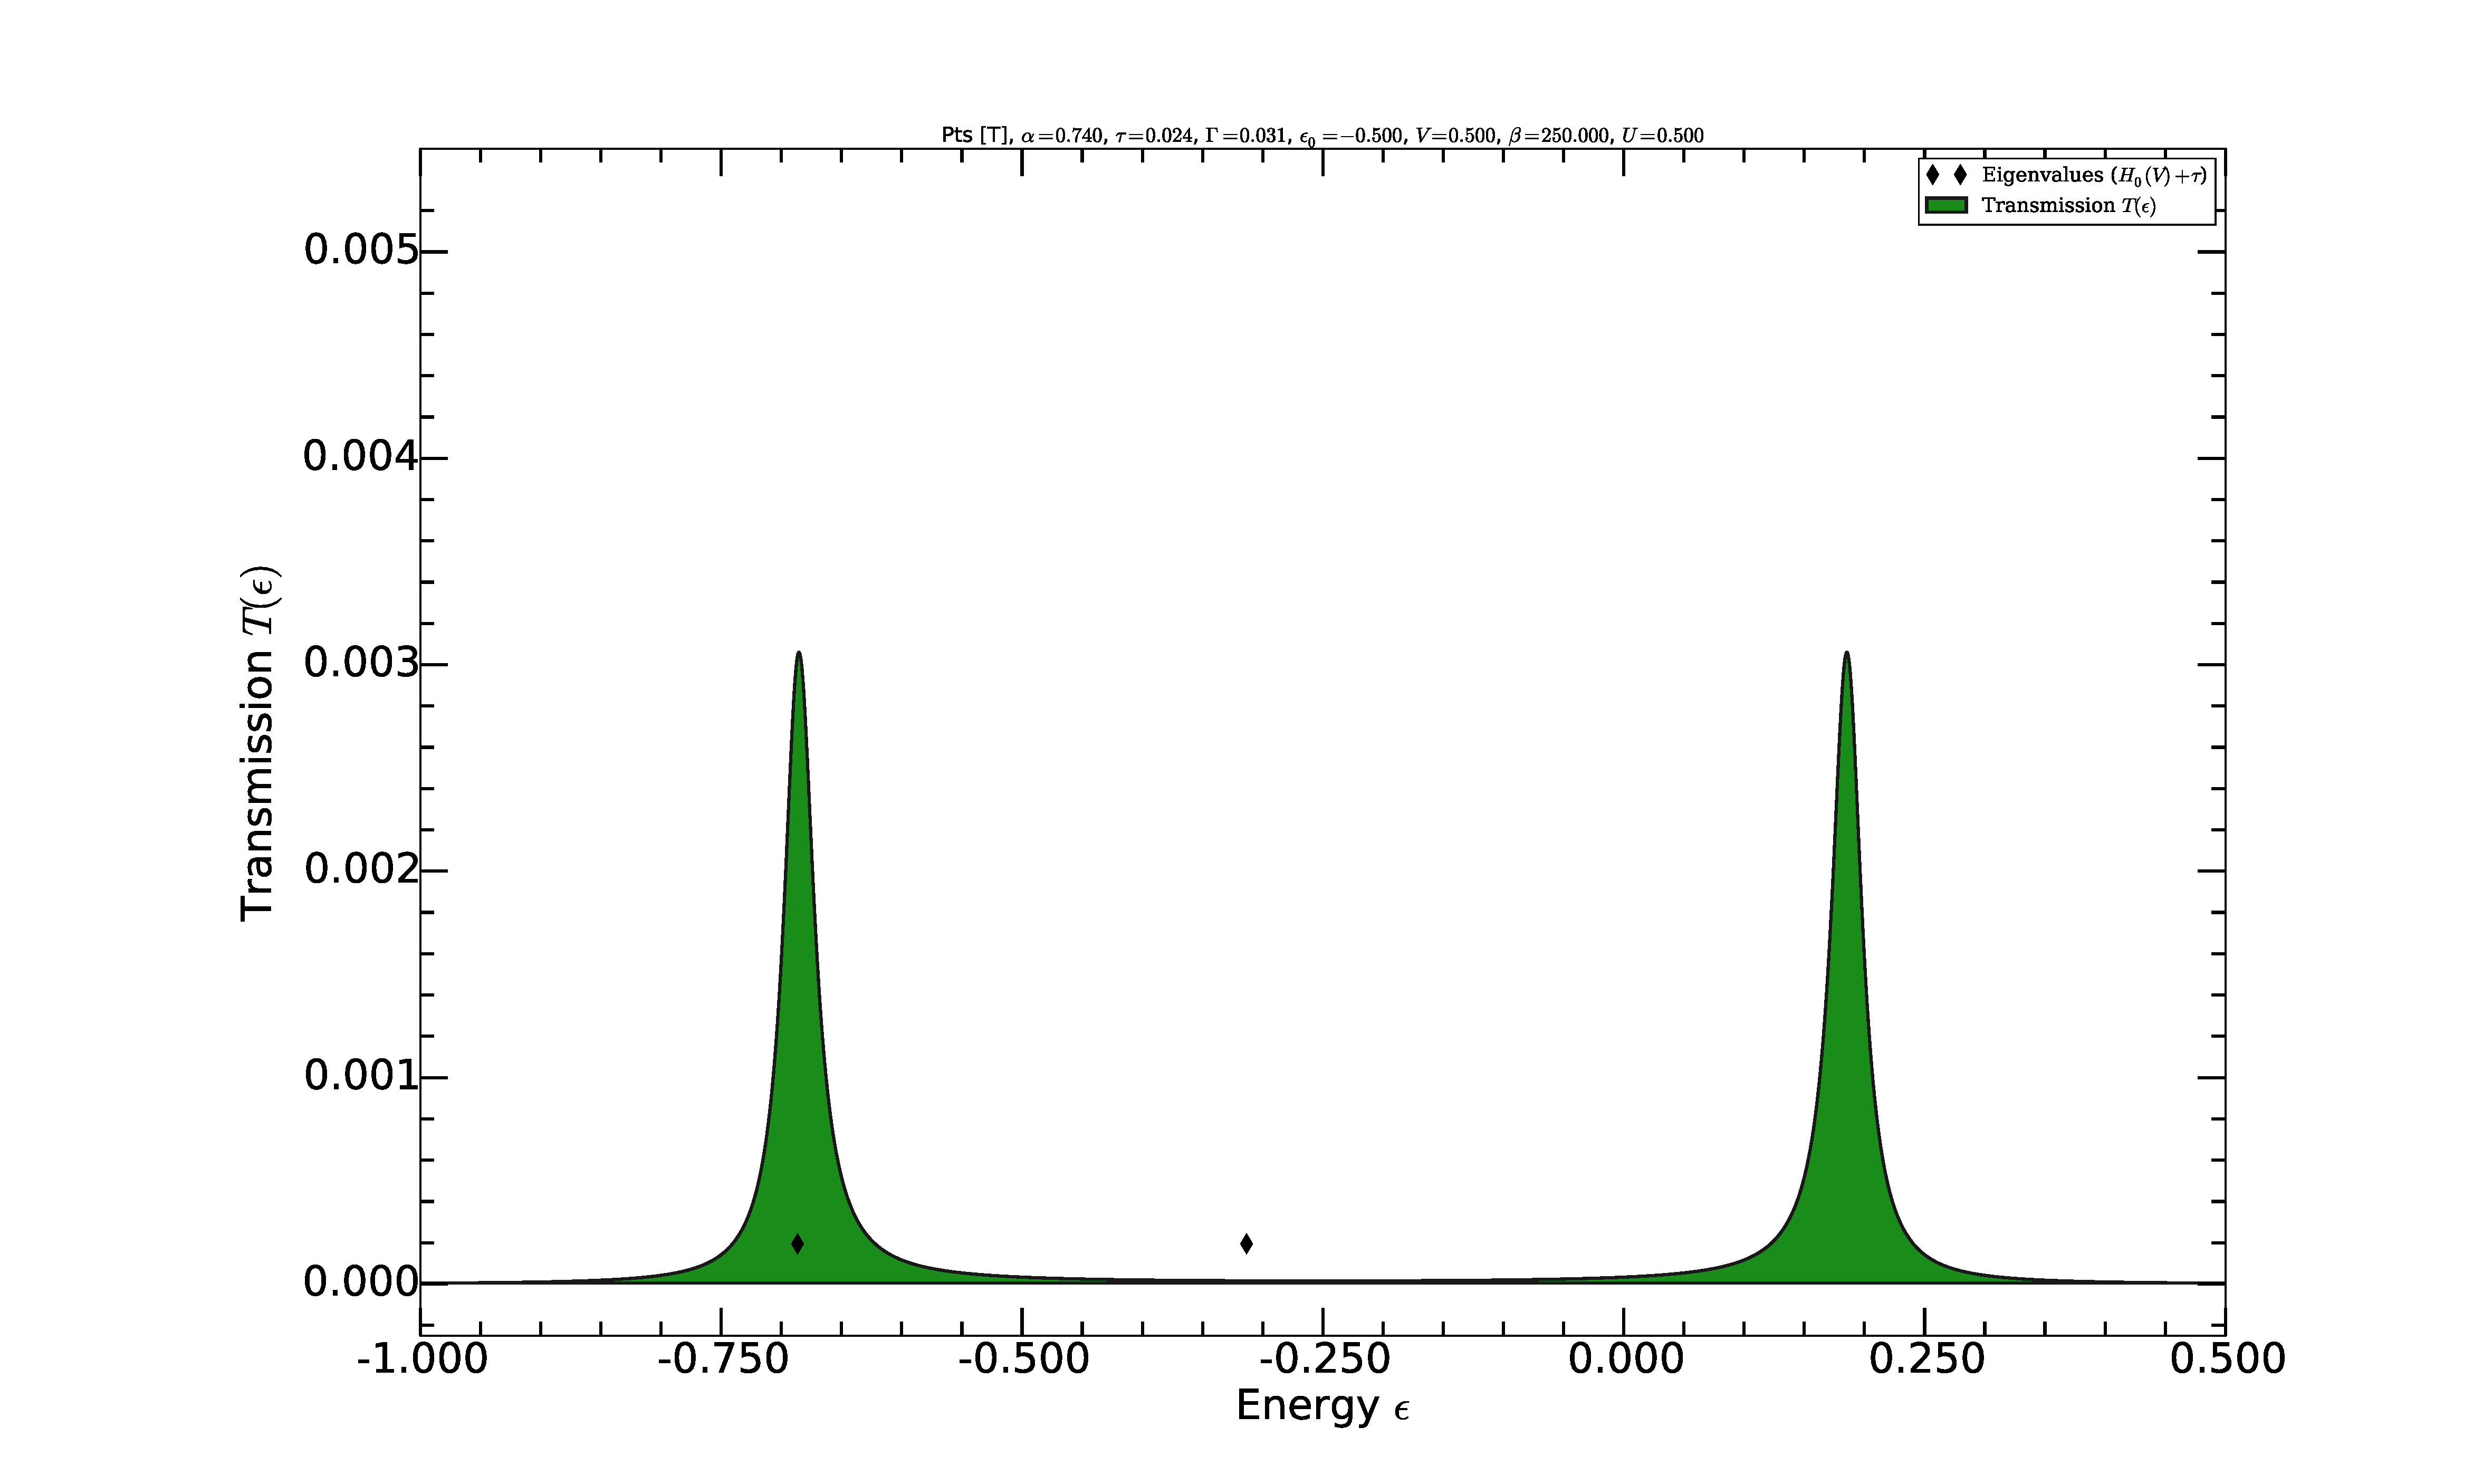
\includegraphics[height=.35\textheight,clip=true,trim=7cm 2cm 7cm 4cm]{pdf/trans/decospinlesstransmissionarbitraryu4.pdf}
    \caption{Transmission spectra for $\alpha=0.74$, $\tau=0.024$, $\Gamma=0.031$, $\epsilon_0 = - 0.05$, $V=0.50$ and $U=0.05$. These parameters are for a strongly-interacting system. In comparison with Figure~\ref{fig:spinlesstransmissionu0} and Figure~\ref{fig:spinlesstransmissionu1}, the peaks have dropped significantly further and the rightmost peak is still exactly $U$ removed from the corresponding eigenvalue.}
    \label{fig:spinlesstransmissionu4}
\end{figure}

All of the figures look as if they are non-interacting two-site spinless models, but the peak values differ. It is perhaps illustrative to consider Figure~\ref{fig:perrin_effective}. In this figure the effective parameters change almost linearly with increasing $U$. The effective parameters are those parameters for which the features of the transmission agree with a non-interacting model ignoring peak height.
\begin{figure}[!bt]
    \centering
    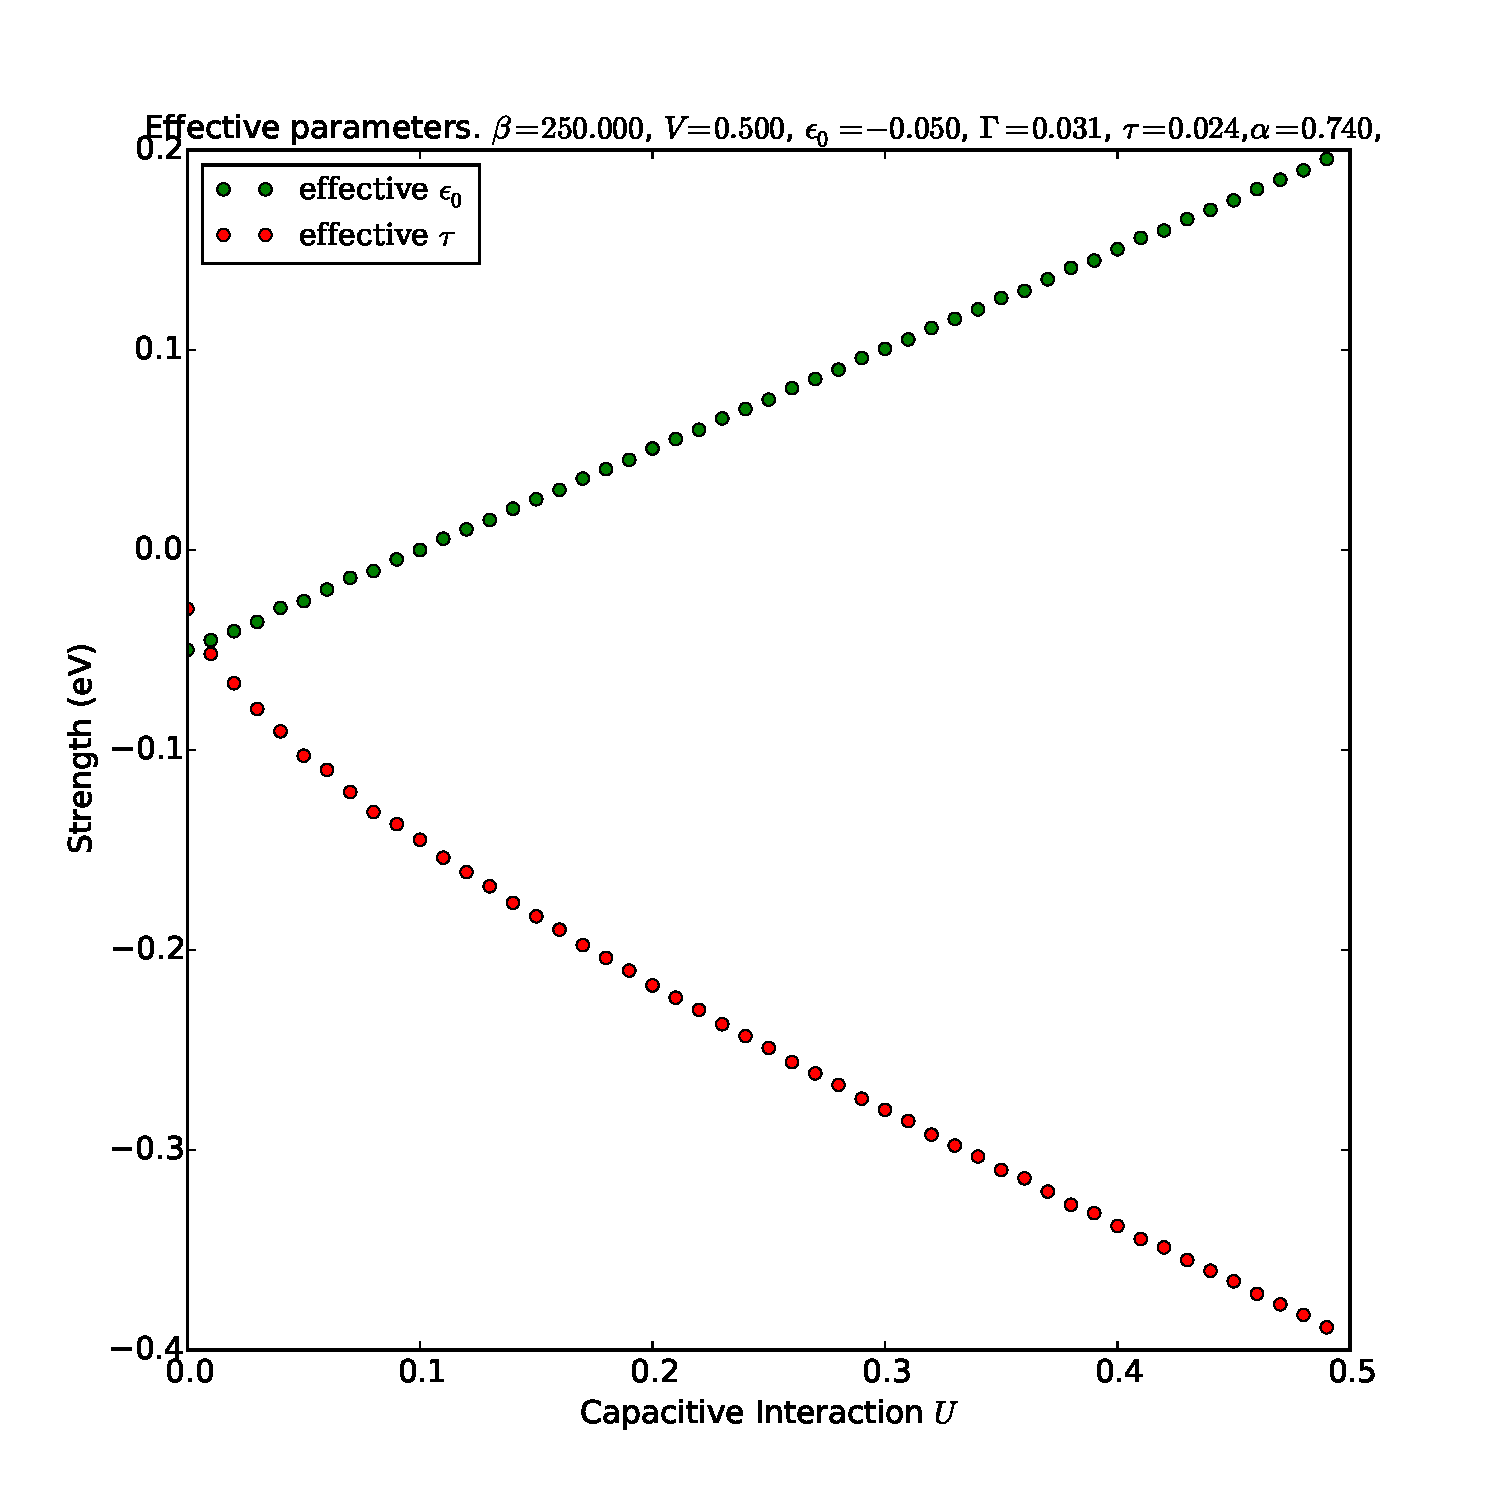
\includegraphics[height=.35\textheight]{pdf/trans/perrin_effective.pdf}
    \caption{In this figure, $\epsilon_0$ and $\tau$ are for a non-interacting model are fitted to an interacting model, leading to `effective' parameters. This ignores the fact that the peaks of an interacting are surpressed. The coupling $\Gamma$ is exactly the same, as is expected.}
    \label{fig:perrin_effective}
\end{figure}


These figures indicate that a mismatch in peak values such as that found in Ref.~\cite{perrinnano} may well be explained in terms of capacitive interaction. Here, the shape would be fitting for a two-site model without capacitive interaction, but the amplitude element of capacitive interaction is merely seen as quantitative disagreement. This notion will be discussed further in section~\ref{sec:perrin}. 

\section{Spinfull two-site model}
I now want to look at the transmission of the spinfull model \emph{in comparison} with that of the spinless model. First, recall that $\zeta$ describes the intersite interaction while $\xi$ the onsite interaction. Given the large amount of possible pictures, here I present only those that are interesting results that are distinct from the spinless model with the exception of Figure~\ref{fig:transmap34} which has extremely strong onsite interaction $\xi$ such that the two models are expected to converge.


First, I want to look at the case where there is no onsite interaction, in which there are two copies of the system and no cross terms; electrons of different spin do not interact. Therefore, we expect the spinfull transmission to be simply twice the spinless transmission. While the occupation of the many-body makes switches, this does not lead to a different set of Green's Functions as $\Sigma^C=0$ for $U=0$. In Figure~\ref{fig:transmap00} we see that this expectation is confirmed. 

\begin{figure}[!bt]
    \centering
    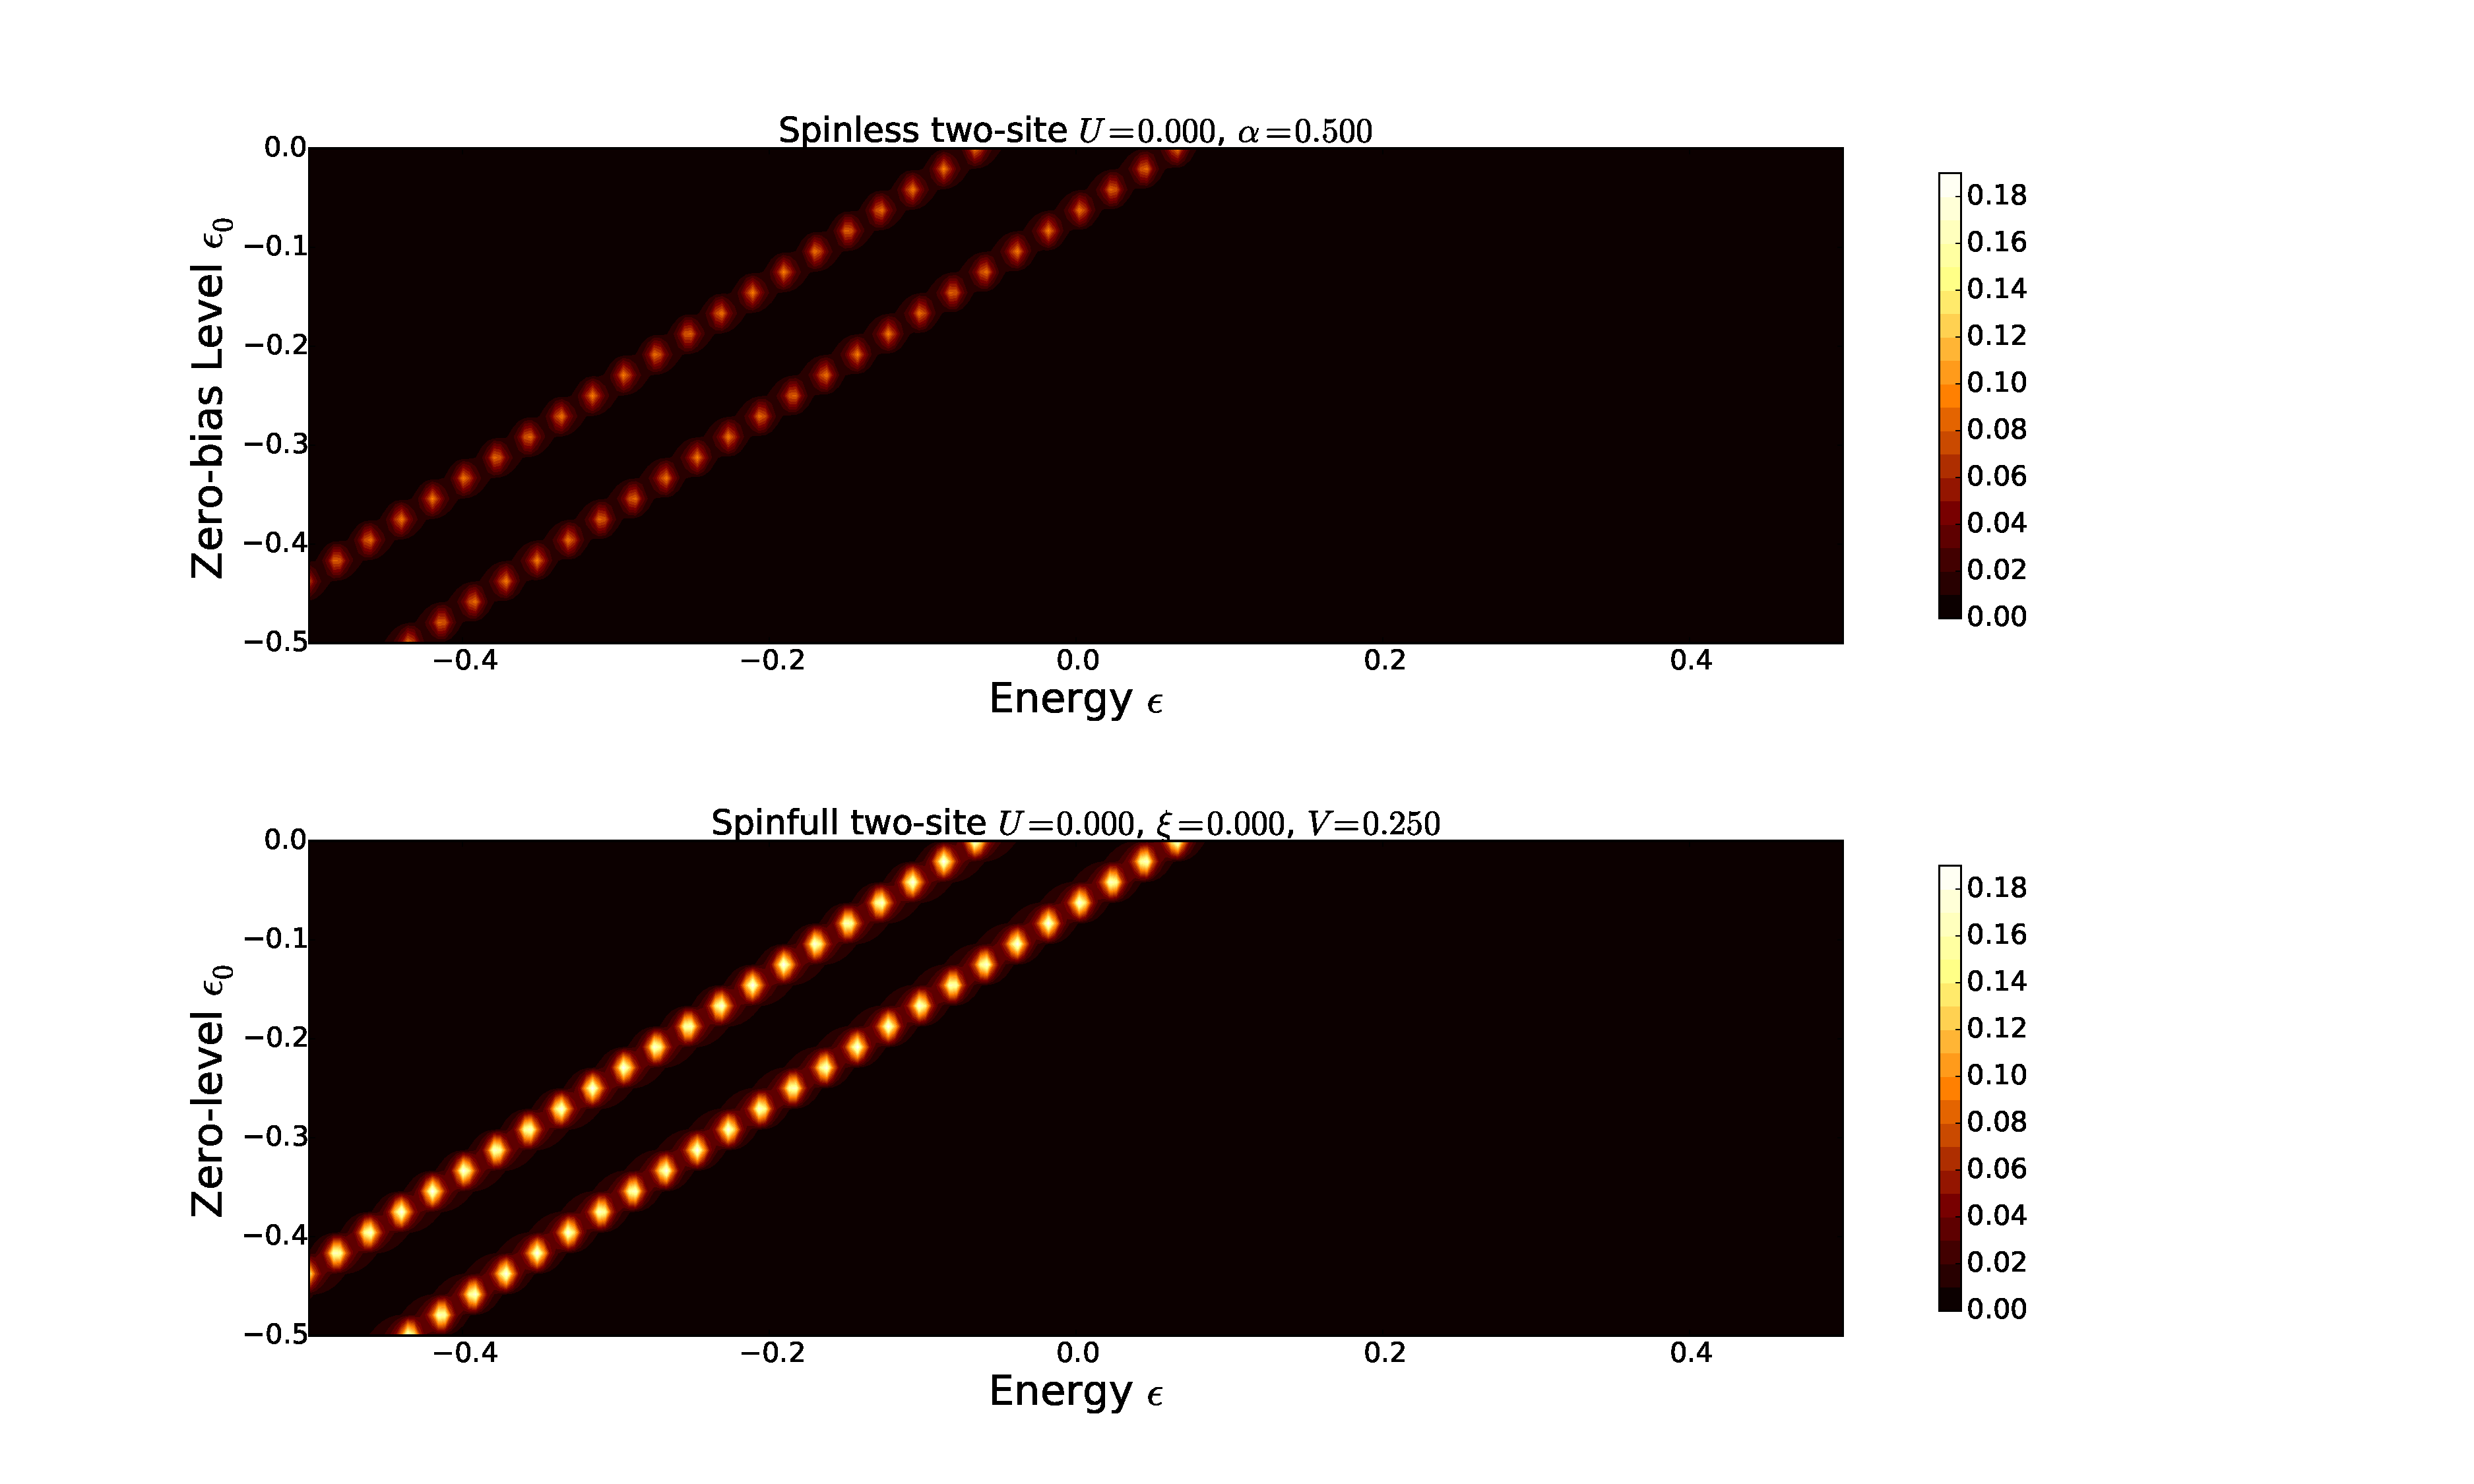
\includegraphics[height=.38\textheight]{pdf/map/transmap_u0_k0.pdf}
    \caption{In this figure, $U=0.00, \zeta=1.00, \xi=0.00$. The two models agree very well, with the spinfull model having two non-interacting copies of the spinless model and thus twice the transmission.}
    \label{fig:transmap00}
\end{figure}
\begin{figure}[!bt]
    \centering
    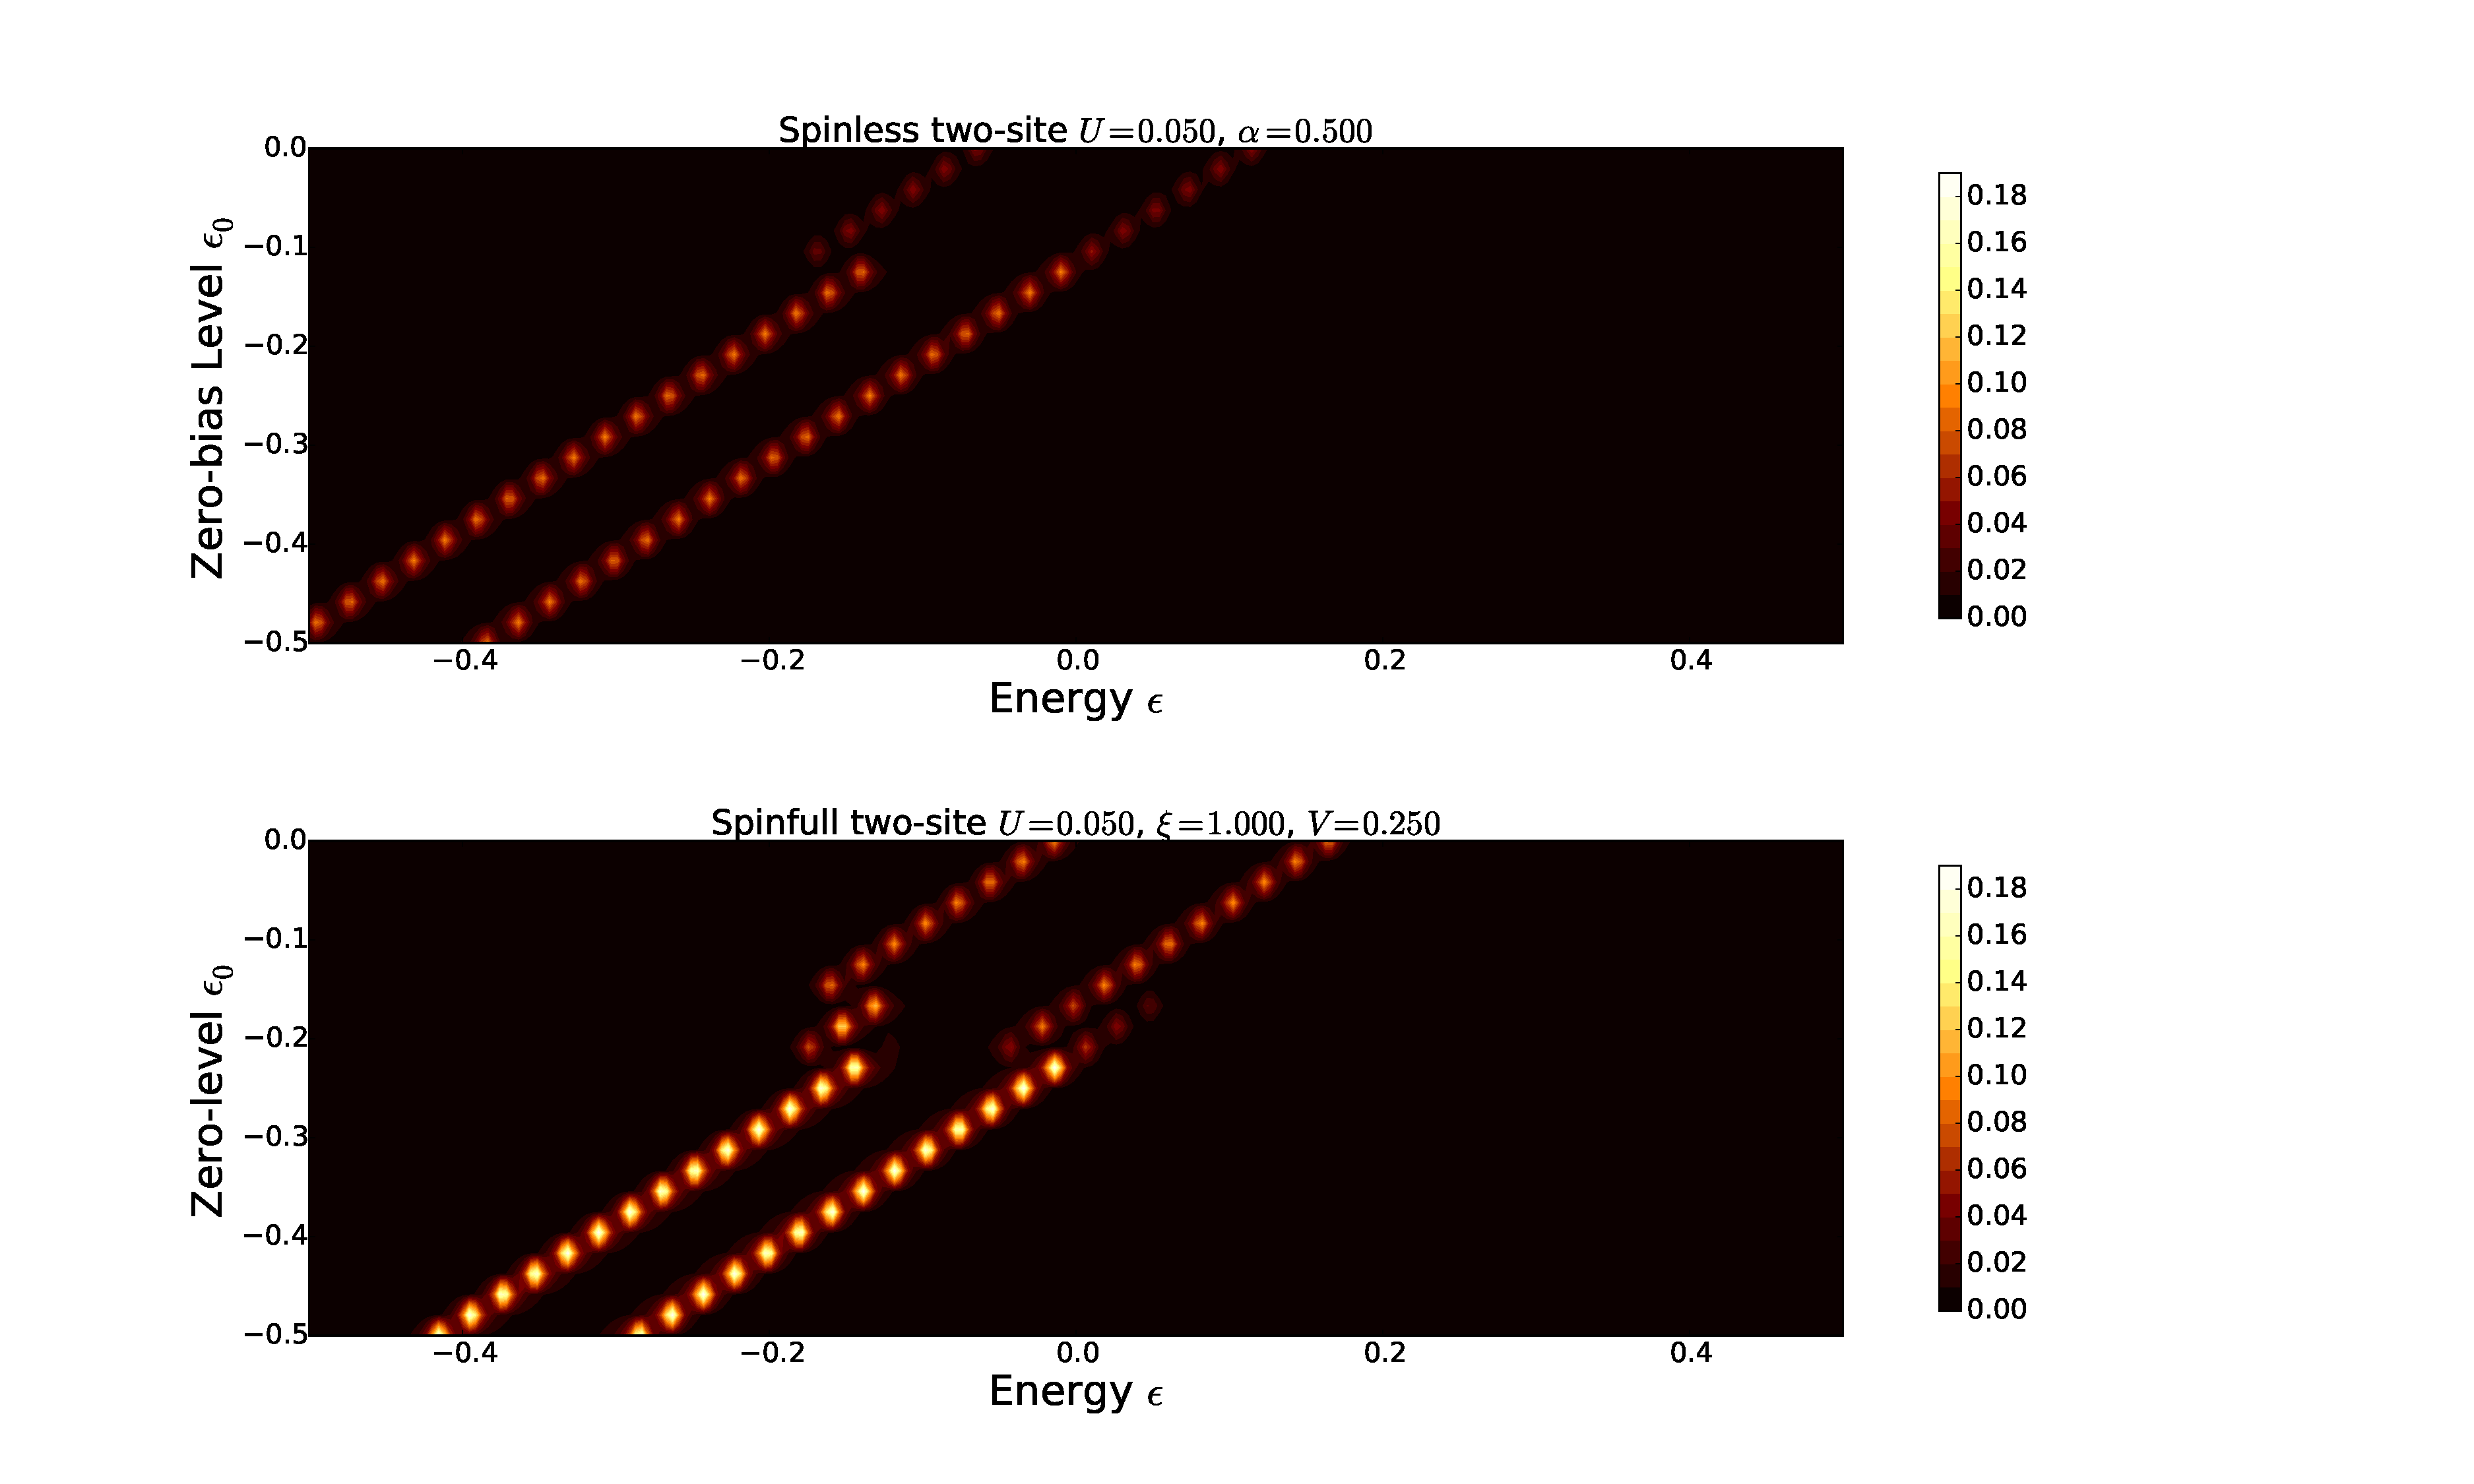
\includegraphics[height=.38\textheight]{pdf/map/transmap_u1_k2.pdf}
    \caption{In this figure, $U=0.05, \zeta=1.00, \xi=1.00$. A distinct difference is very clear, with a three-peak transmission spectrum making a short appearance. See the main text for explanation.}
    \label{fig:transmap12}
\end{figure}
\begin{figure}[!bt]
    \centering
    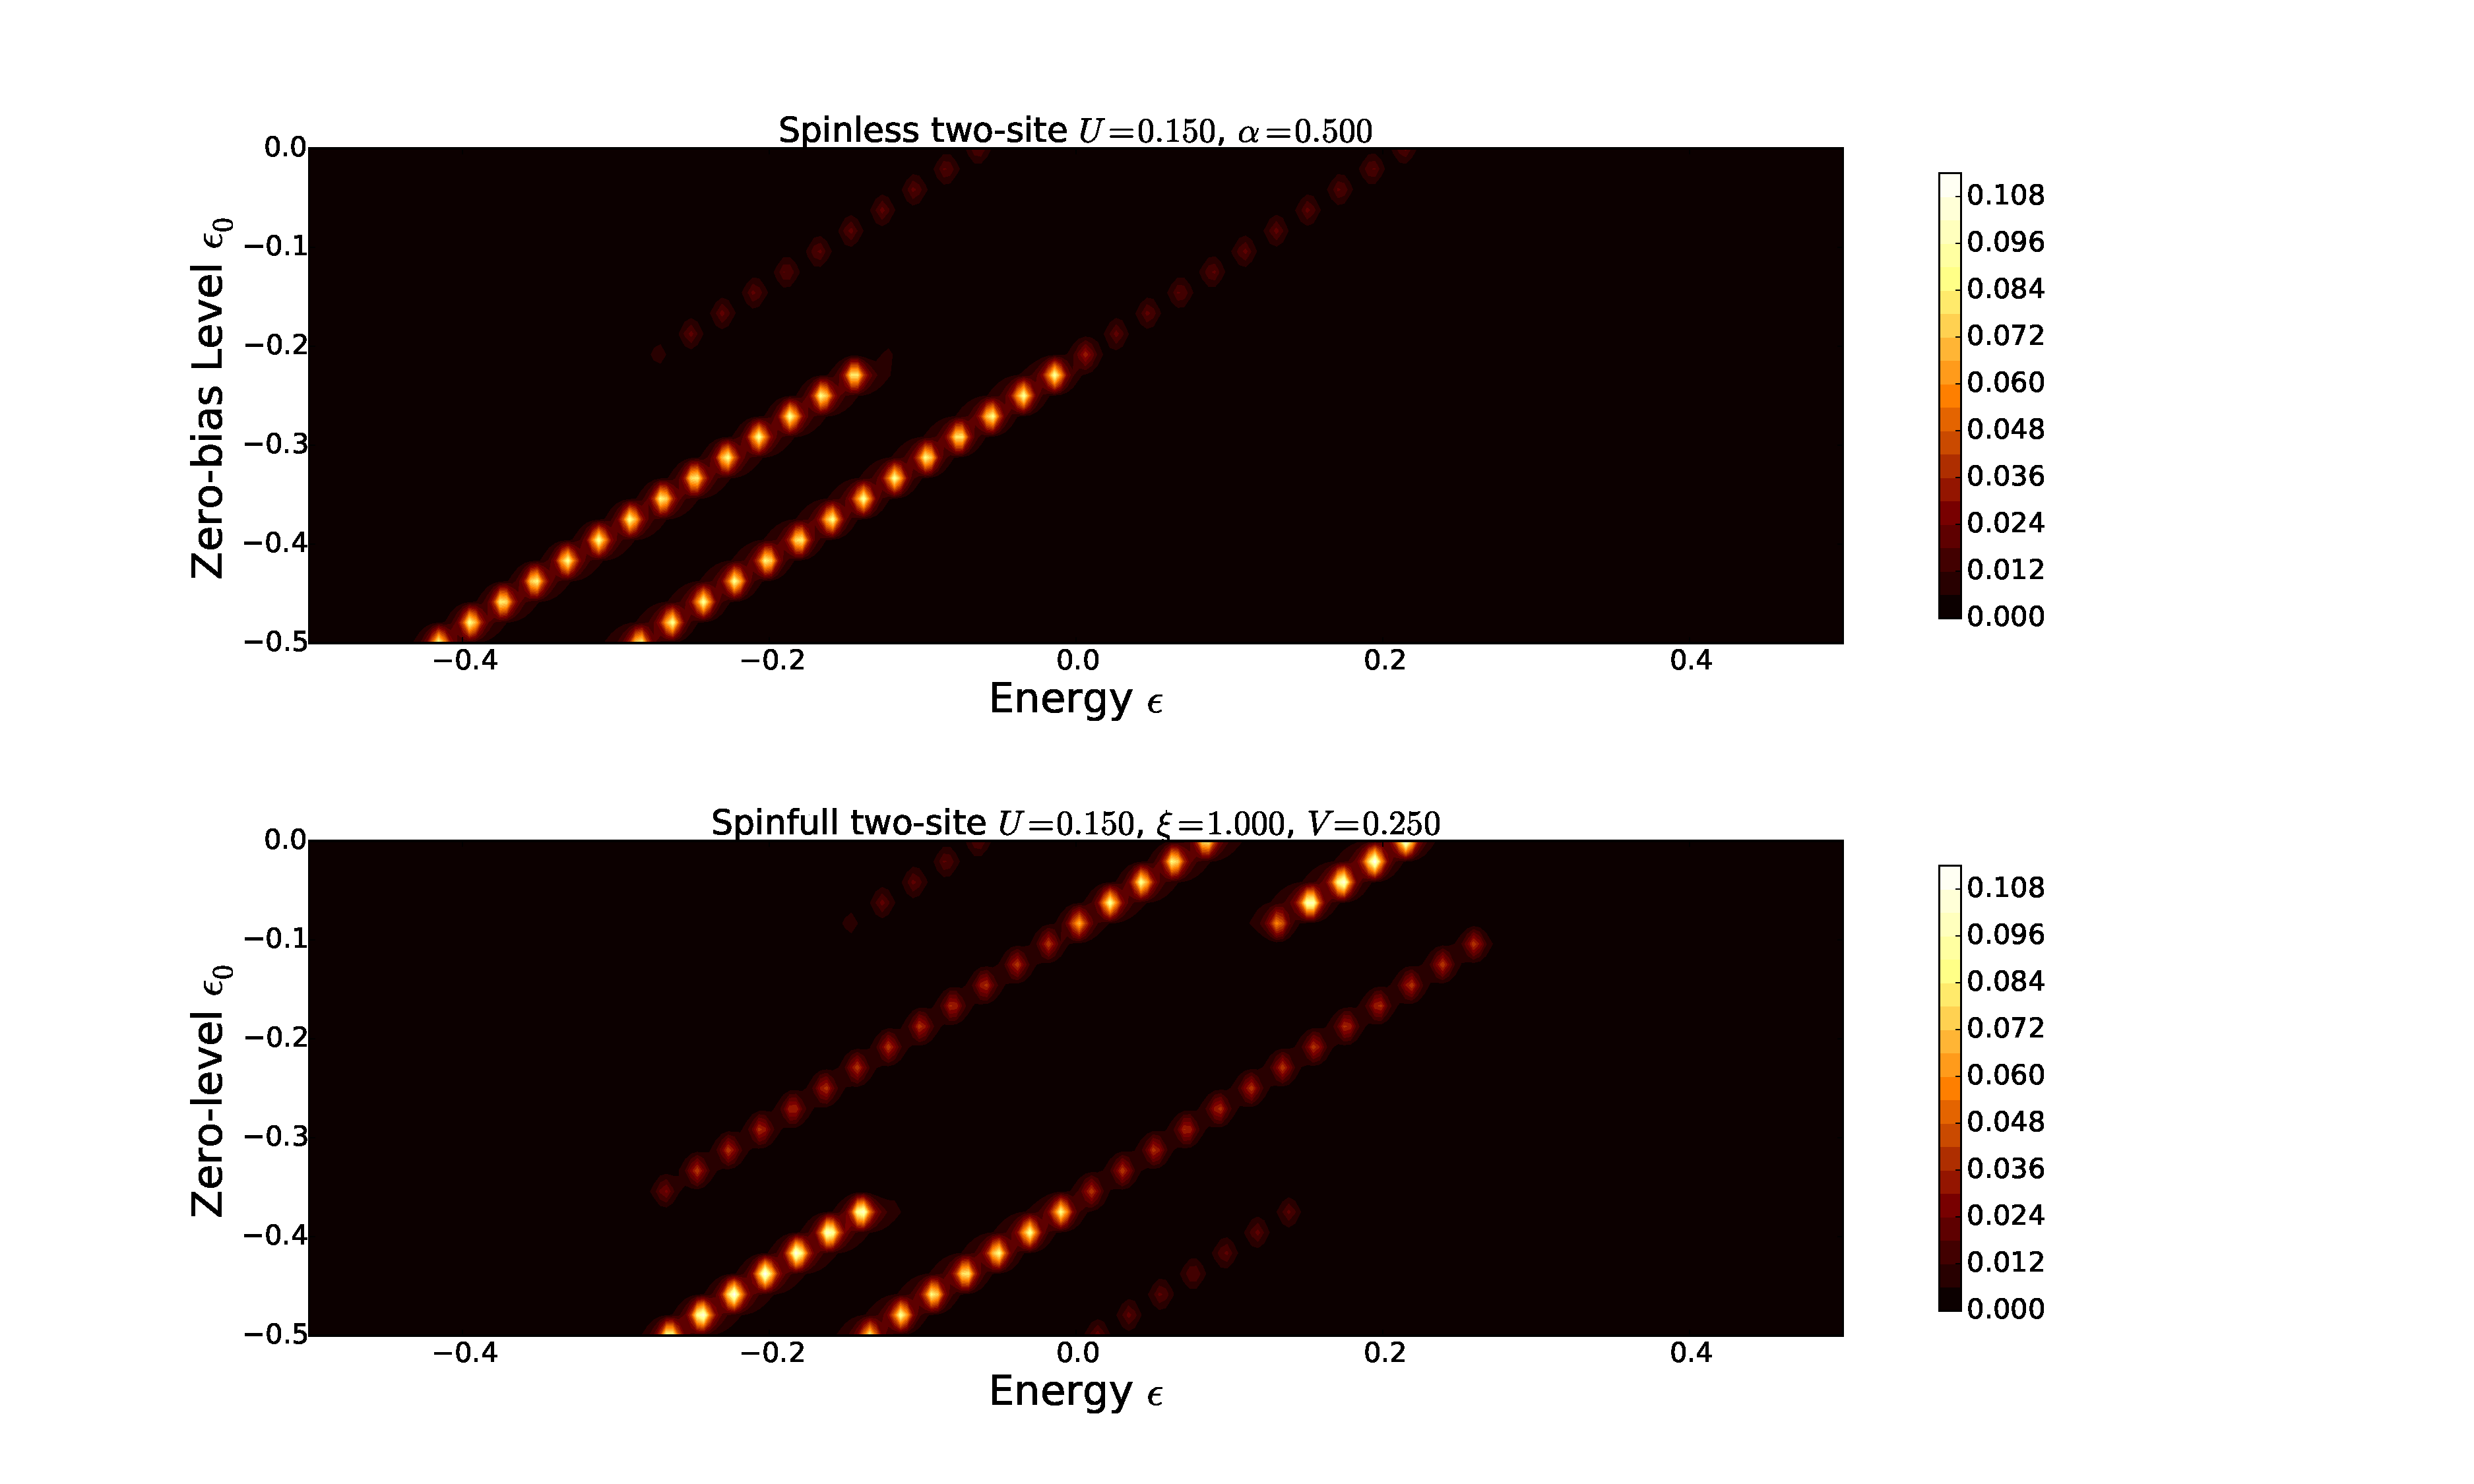
\includegraphics[height=.38\textheight]{pdf/map/transmap_u2_k2.pdf}
    \caption{In this figure, $U=0.15, \zeta=1.00, \xi=1.00$. There is a very obvious difference, with three peak transmission spectra dominating the spinfull results. See the main text for explanation.}
    \label{fig:transmap22}
\end{figure}
\begin{figure}[!bt]
    \centering
    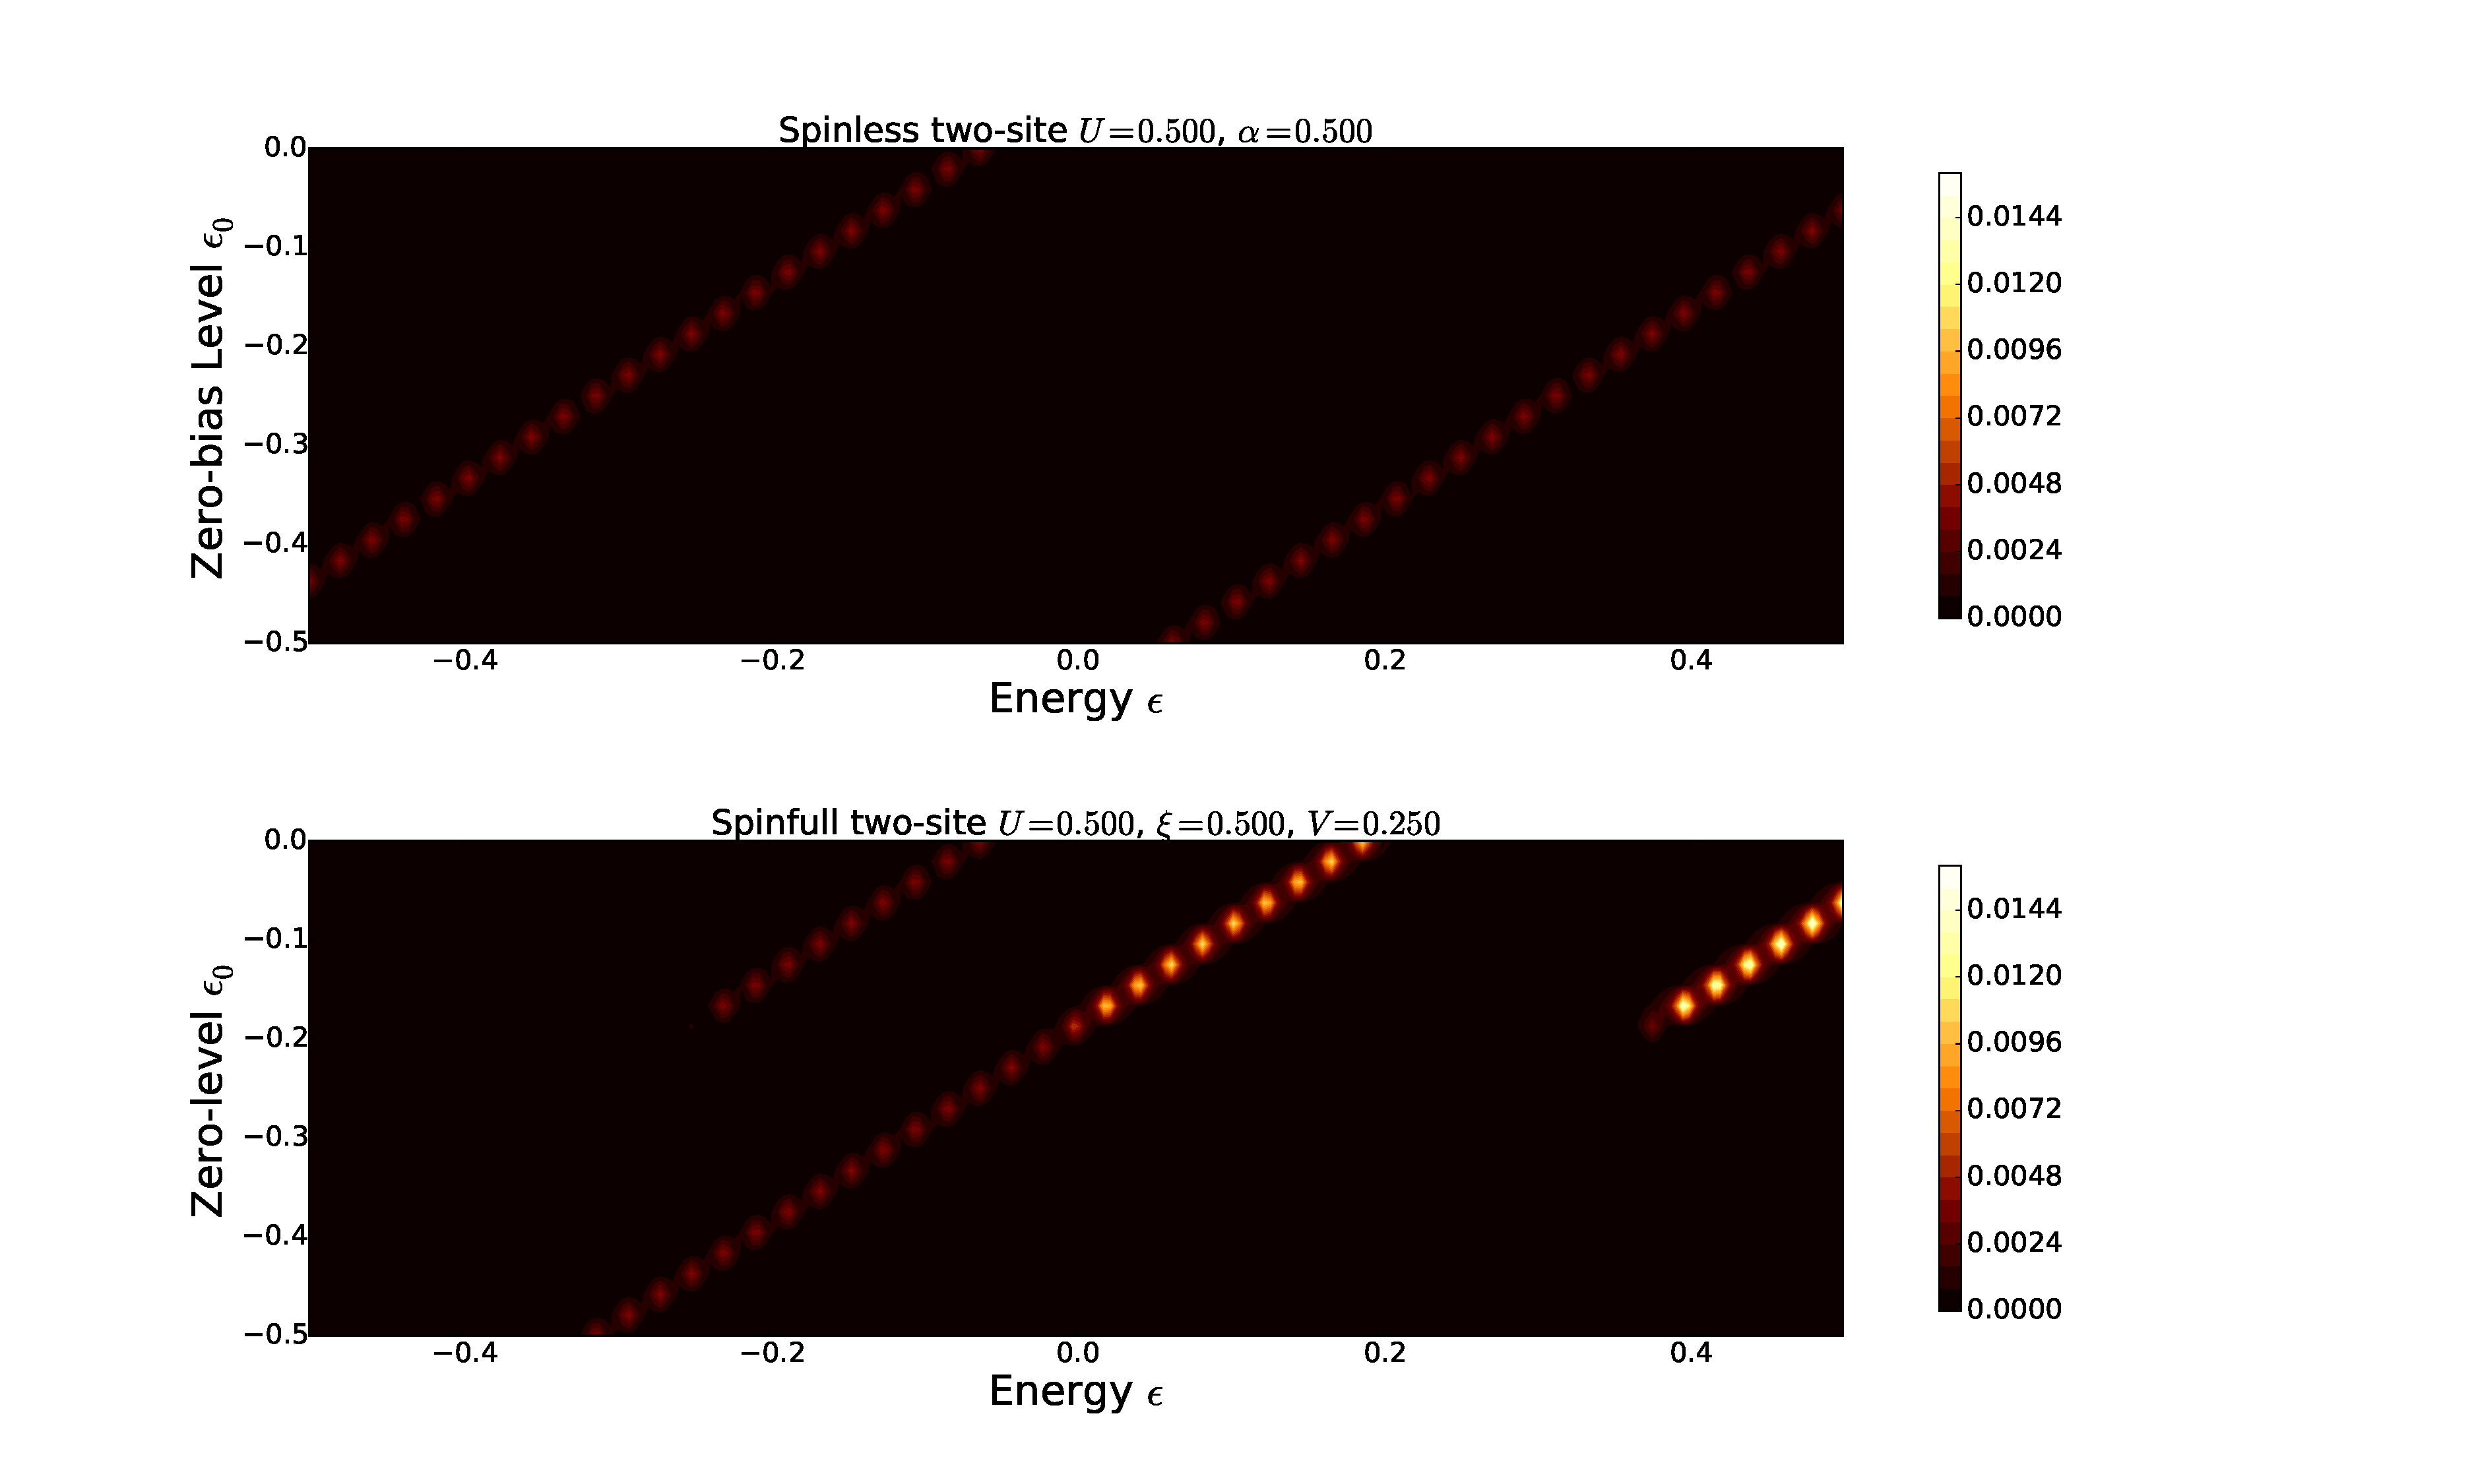
\includegraphics[height=.38\textheight]{pdf/map/transmap_u3_k3.pdf}
    \caption{In this figure, $U=0.15, \zeta=1.00, \xi=1.00$. The is a very pronounced difference, with three transmission peaks above $\epsilon\approx -0.2$ and only a single peak below that level.  See the main text for explanation.}
    \label{fig:transmap33}
\end{figure}
\begin{figure}[!bt]
    \centering
    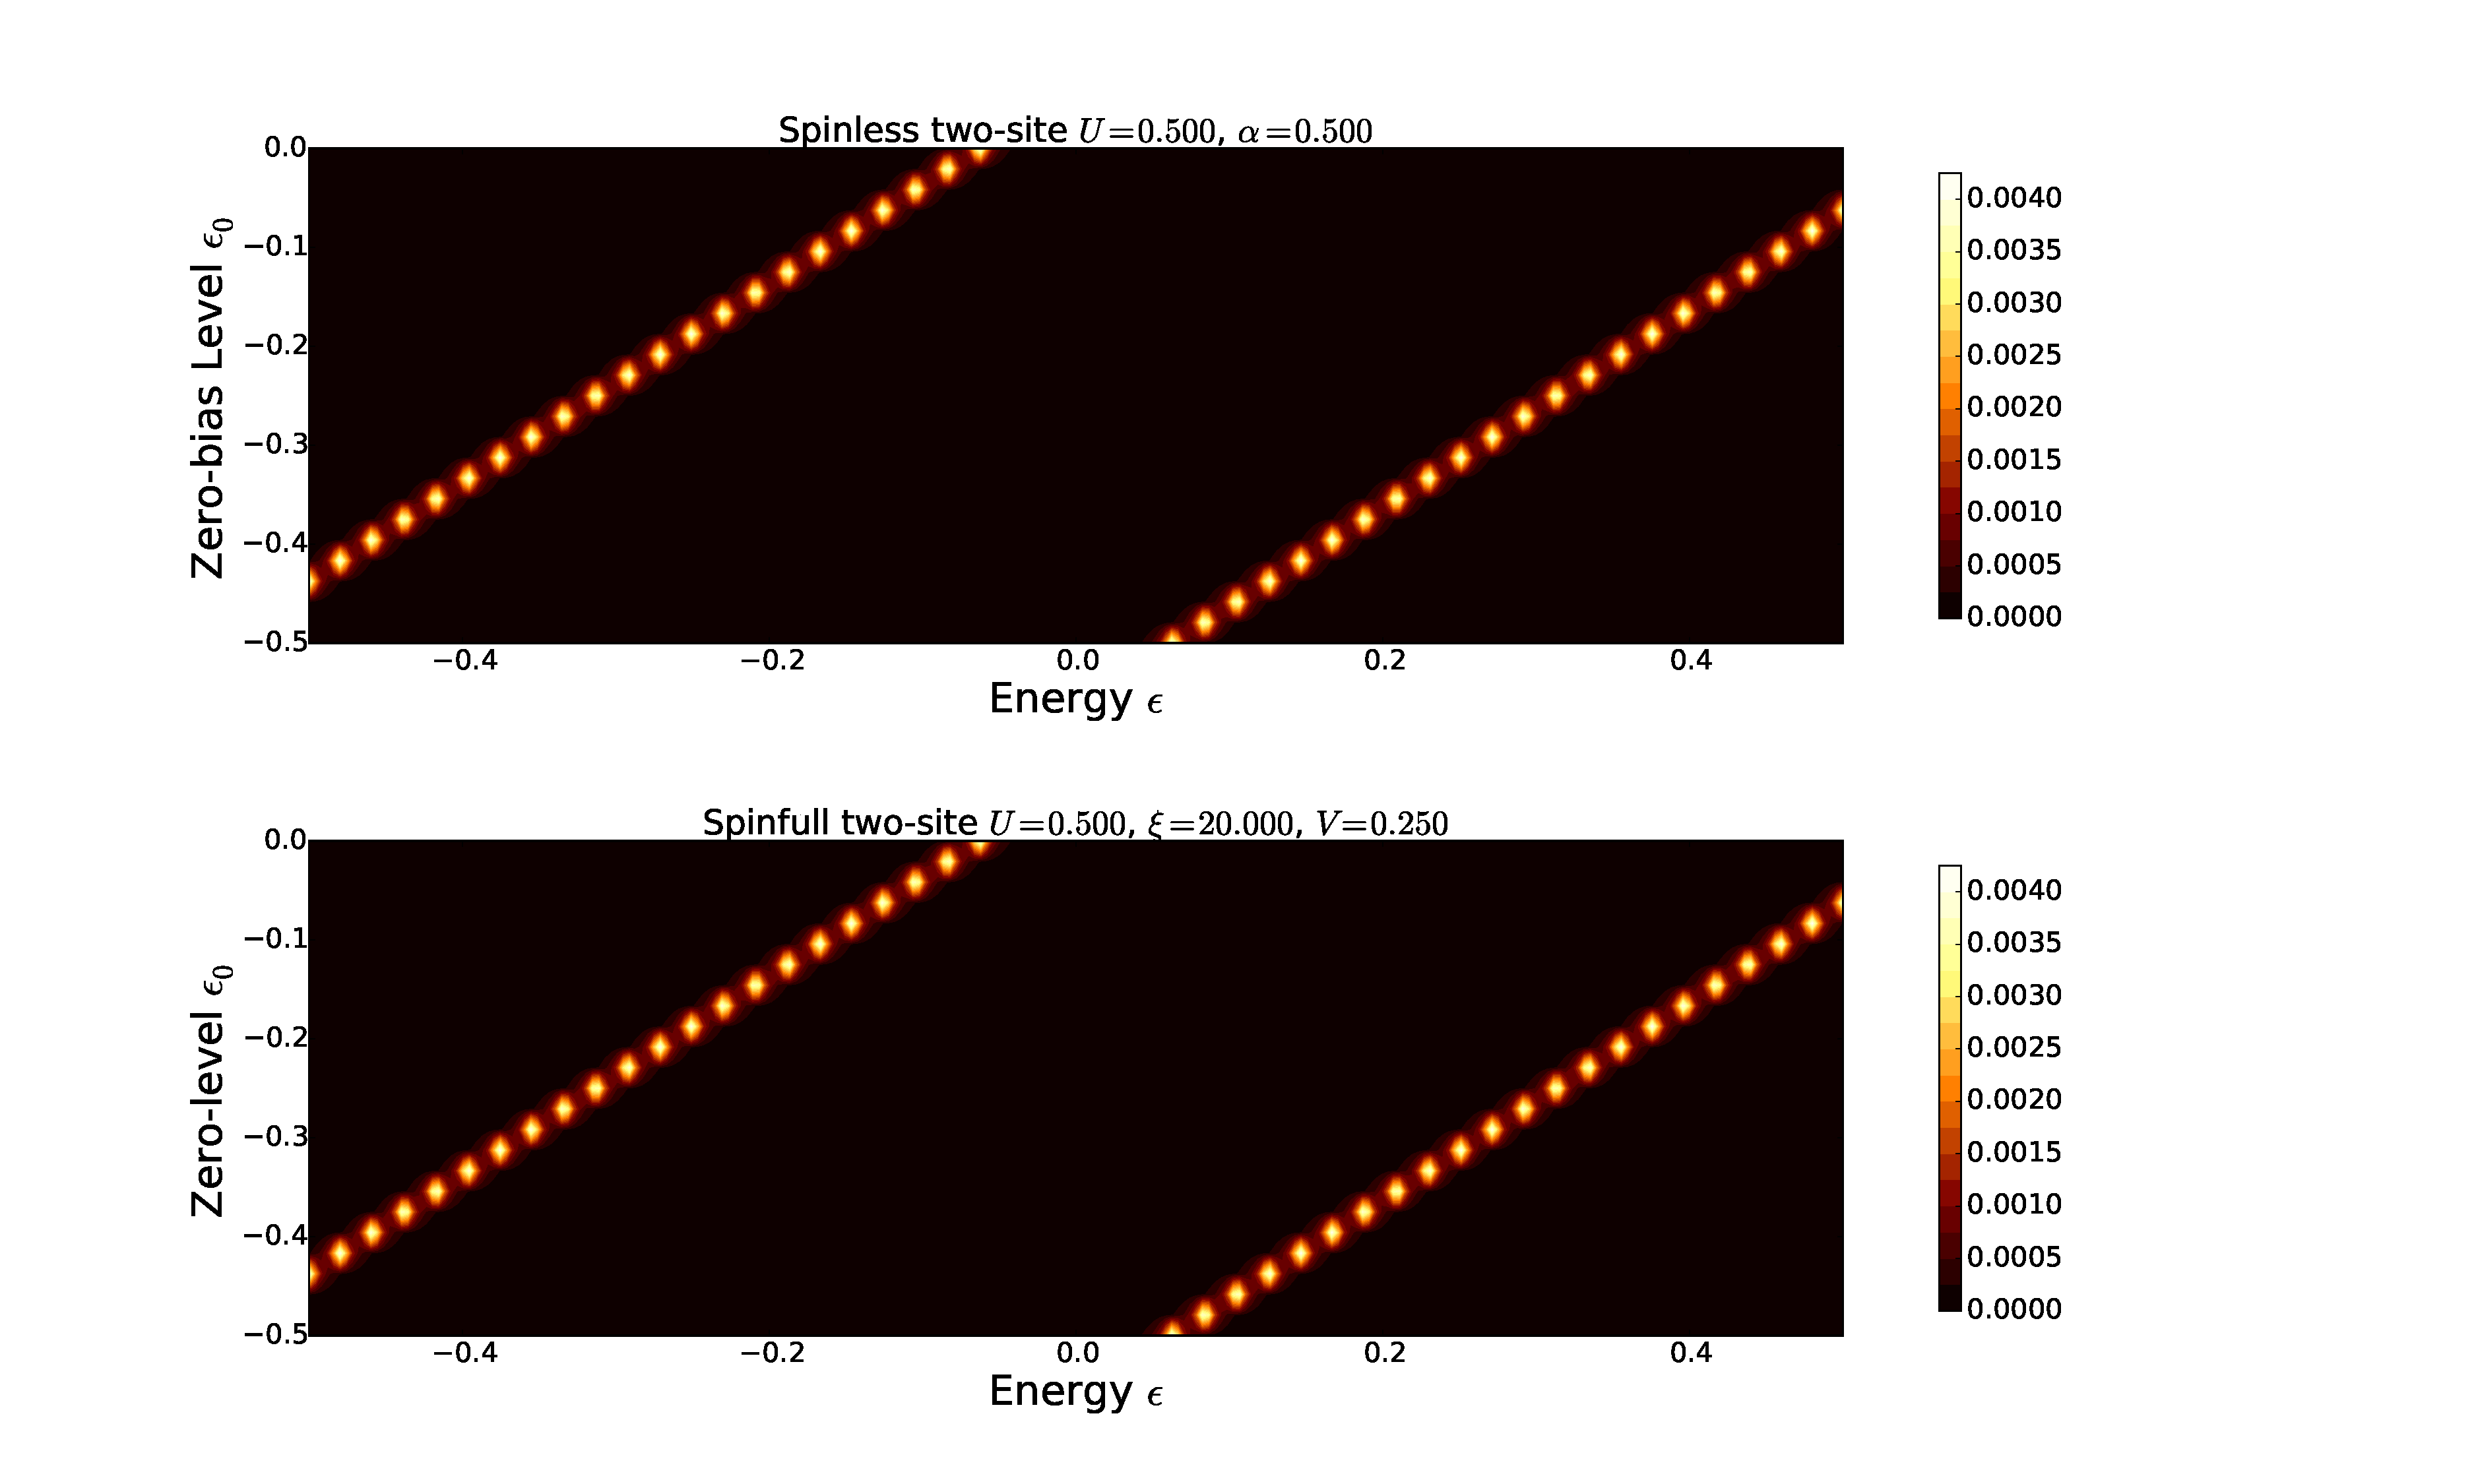
\includegraphics[height=.38\textheight]{pdf/map/transmap_u3_k4.pdf}
    \caption{In this figure, $U=0.15, \zeta=1.00, \xi=1.00$. The two models converge, which is expected for this $\xi$. See the main text for explanation.}
    \label{fig:transmap34}
\end{figure}

Evidence of the many-body character of both models is clear in Figure~\ref{fig:transmap12}, where there is one switch in transmission peaks for the spinless model and two switches for the spinfull model. The spinless model switches from $\ket{01}$ to $\ket{11}$ (Figure~\ref{fig:perrinenergy1}), displacing one peak by an amount $U$ which agrees well with the transmission figure.  The spinfull model, on the other hand, switches from $\ket{0011}$ to either $\ket{0111}$ or $\ket{1011}$ before switching to $\ket{1111}$ (Figure~\ref{fig:perspinenergy12}). Note that the rightmost peaks corresponds to the left site, and the leftmost peak corresponds to the right site. The first switch displaces the leftmost peak\footnote{Adding an electron to the left level adds $U$ to the right level, which displaces the left peak.}and seems to have placed a third peak at the rightmost peak plus $U$, a likely result because the energy states are degenerate. The second switch then displaces the leftmost peak by $\xi U$. 

Figure~\ref{fig:transmap22} is simply explained for the spinless model in terms of the many-body switches. The spinfull model is slightly more involved. Figure~\ref{fig:perspinenergy22} shows that the state is degenerate for $\epsilon_0 \gtrsim -0.1$, that the degeneracy is lifted initially but that it again becomes degenerate after $\epsilon_0 \lesssim -.36$. The degeneracy is clear in the transmission, because one of the \emph{three} peaks is weaker than the other two. 

Figure~\ref{fig:transmap33} is more simply explained. Figure~\ref{fig:perspinenergy33} indicates that 


\section{Current parameter sweeps}
\label{sec:twositeparamsweep}
\section{Experimental fit}
\label{sec:perrin}
%clearpage dumps all images in the stack. Also prevents images from skipping chapters.
\clearpage
\references{dissertation}